\documentclass[12pt]{report}
\usepackage[a4paper, left=2.5cm, right=2.5cm, top=2.5cm, bottom=2.5cm]{geometry}
\usepackage{graphicx}
\usepackage{listings}
\usepackage{color}
\usepackage{multirow}
\usepackage{tabularx}
\usepackage[hidelinks]{hyperref}
\hypersetup
{
	colorlinks=false,
    linktoc=all
}

\graphicspath{ {images/} }



% Code fragment formatting
\definecolor{dkgreen}{rgb}{0,0.6,0}
\definecolor{gray}{rgb}{0.5,0.5,0.5}
\definecolor{myRed}{rgb}{0.64,0.082,0.082}

\lstset{
	frame=tb,
	language=[Sharp]C,
	aboveskip=1mm,
	belowskip=1mm,
	showstringspaces=false,
	columns=flexible,
	basicstyle={\scriptsize\ttfamily},
	numbers=left,
	numberstyle=\tiny\color{gray},
	keywordstyle=\color{blue},
	commentstyle=\color{dkgreen},
	stringstyle=\color{myRed},
	breaklines=true,
	breakatwhitespace=true,
	tabsize=4
}

\begin{document}

\begin{titlepage}
	\begin{center}		
		\vspace*{5cm}
		\textbf{\LARGE{Vehicle Self Diagnosis Application}}\\
		\vspace{6cm}
		\large{		
		\textbf{Name:} James Preston\\
		\textbf{ID:} 12159247\\
		\textbf{Course:} LM110 - Computer Games Development\\
		\textbf{Supervisor:} Mr. J.J. Collins\\
		\textbf{Date:} 18\textsuperscript{th} March 2016 \\
		}
	\end{center}
\end{titlepage}

	\tableofcontents
	\newpage
	
	\chapter{Introduction}
		\section{Summary}
	\paragraph{}{
	This project is focused on the development of an application capable of communicating with a vehicle and providing feedback on potential issues with it. The information that the application gathers can then be used by the end user when negotiating guesstimates on service charges with professionals, such as mechanics. The intention is that an end user with no technical or mechanical knowledge about their car can perform a self check to get an estimation of the severity of the issues with the vehicle along with the cost associated with fixing them.
	}
	\paragraph{}{
	The project will provide a number of benefits for the target audience: the average vehicle owner. Firstly, it will provide them with a better knowledge of the state of their vehicle. They will be able to use this information to obtain a better knowledge of the inner workings of their vehicle and to determine if the car needs a check up in the near future. It will also save the end user time and money, by allowing them to self check the car rather than paying for a professional to do it for them.
	}
	\paragraph{}
	{
	The architecture of the application will be highly extensible allowing for new functionality to be added with relative ease. It will also allow for the application to be ported to other operating systems, such as Android and iOS. The extensibility of the architecture of the application will be evaluated by porting a subset of the features to Android. This will be accomplished using the Xamarin Framework, which allows for writing Android and iOS applications using C{\#}.
	}
	\paragraph{}
	{
	The application will be evaluated through field testing by connecting to live vehicles. This testing will involve establishing and maintaining communications with the vehicle and gathering the relevant data from it. The data gathered will then be compared to that of similar applications to verify that the application functions correctly.
	}
	
\section{Overview of Domain}
	\paragraph{}{
	Over the years, cars have been transformed from purely mechanical tools to more sophisticated technical machines. Most modern vehicles now contain built in computers, called Engine Control Units (ECU), that monitor and control its various subsystems, for example the Anti-lock Brake System (ABS). As the complexity of vehicles grew, it became harder to track defects. While issues in earlier vehicles could be narrowed down to a mechanical failure, modern vehicles can have mechanical or electrical faults. Now, all modern vehicles have an On-board Diagnostics (OBDII) port, which allows diagnostic tools to connect to the vehicle. The OBDII standard also defines a subset of data that must be retrievable from all compliant vehicles, and the messaging format of the data.		 
	}
	\paragraph{}{
	The application will use an ELM327 Bluetooth dongle to connect to and communicate with the vehicle. This is a micro-controller that connects to the OBDII port found in modern vehicles. The ELM327 abstracts the communication process by including it's own commands that are passed to the vehicle. This removes the need for low level communication between the application and the vehicle. The ELM327 also has a number of benefits for the end user. Firstly, they are inexpensive and widely available, meaning the end user doesn't have to spend time or money sourcing the device from a specific vendor. The device also requires no setup, as the application will handle this automatically. Overall, the ELM327 benefits the developer by having a universal communication system, and benefits the end user by being cheap and easy to use.
	}
	\paragraph{}{
	The application will be developed as a Windows Universal App. With the release of Windows 10, Microsoft allowed developers to create applications that would run on all Windows 10 devices. While a similar concept was seen with Windows 8.1, these applications only require a single codebase. This provides the developer with the ability to deploy on multiple devices, such as phones, laptops and tablets, while also promoting maintainability of the code. It made sense to create an application for Windows, as it is the de facto standard operating system for home users, with all distributions of Windows holding a combined share of over 88{\%} of the operating system market share %\cite{OSMarketShare}.
	}
	\paragraph{}{
	As the application is Windows based, portability is an issue, as it would require a partial or full rewrite of the code to port it to Android or iOS, which is impossible given the timeframe of this project. Fortunately, the Xamarin framework allows for the creation of native applications for Android and iOS, using the C{\#} language. This means the code written for the existing application may be used for an Android port, with only a new UI needing to be created. This feature is of great importance to the project, not only to demonstrate the portability of the code, but to target more users.
	}
		
\section{Objectives}
	\paragraph{}{
	The key objectives that have been identified for this project are as follows:
		\begin{itemize}
			\item \textbf{Allow users to retrieve diagnostic information from their vehicle}\\
			The primary objective of this project is to create an application that will allow a user to communicate with and retrieve information from their vehicle. However, it is of paramount importance that the application is easy to use and comprehend without the user having any technical knowledge of their vehicle.
			
			\item \textbf{Develop a highly extensible and portable system}\\
			A key goal of the project is the design and implementation of an extensible and portable architecture. This is to allow	the application to be easily expanded in future and to be deployed on numerous platforms to target a larger user base.

			\item \textbf{Ensure the system cannot cause damage to a vehicle}\\
			As the system is designed for use by non-technical stakeholders, there is a risk that they may misuse the application due to a lack of technical knowledge. The system must account for this during the design and implementation stages.
		\end{itemize}
	}
	
	%\paragraph{}{
	%The primary objective of this project is to create an application that will allow a user to communicate with and diagnose their vehicle. However, it is of paramount importance that the application is easy to use and comprehend without the user having any technical knowledge of their vehicle.  
	%}
	%\paragraph{}{
	%The most challenging aspect will be finding a balance between the correct level of abstraction for an average user to understand, whilst also providing enough detail that they have all the information they need to perform a diagnosis. There are existing applications that provide similar services, but they are more directed at mechanics and repair technicians, who have an in depth understanding of the technical aspects of vehicles.
	%}
	%\paragraph{}{
	%The secondary objective will be to gain experience working with new technologies such as the design and development of Windows 10 Universal Apps. This will involved learning how to use C{\#} and XAML for development and researching the UI design guidelines for Windows Universal Apps to ensure the application has the aesthetics and usability that it is expected of modern applications.
	%}
	
\section{Methodology}
	\paragraph{}{
	This project will follow a Scrum development process, operating on week long sprints, including a retrospective with the project supervisor at the end of the week.
	}
	\paragraph{}{
	Planning will take place at the start of the project. During this phase, a project roadmap will be created, outlining the tasks and deliverables for each sprint. However, as requirements change and new information comes to light, it will be important to update the project plan over the course of the development cycle. This will occur during the retrospective, if necessary.
	}
	\paragraph{}{
	The basic system architecture will be designed at the start of the project. The intention is to create an extensible, modular architecture and the lightweight upfront design will provide a template to follow throughout the development cycle. After the basic architecture has been designed, all further design work will be done on a per module basis. This includes system and UI design work.
	}
	\paragraph{}{
 	The approach to implementation will be similar to that of design. A basic proof of concept and some prototypes will be created at the start of the project, before moving to an iterative approach. There will be a focus on writing code that has high readability and reusability. The code will be stored in a source control repository, to ensure that a backup is always available, and to keep track of code changes. Testing is an important aspect in the project, so unit tests will be written that will run before committing code to the source control repository. The application will undergo field testing as mentioned above. A variety of vehicle makes and models will be tested to find any defects and ensure the application functions as expected. 
	}

\section{Motivation}
	\paragraph{}{
	In recent years, it has become more commonplace for end users to self diagnose issues with their personal belongings. If an end user has an issue with a laptop or phone, they will usually search the internet for more information about the severity of the issue, rather than contacting the customer care service directly. This project intends to allow end users to apply that process to issues with their cars.
	}
	\paragraph{}{
	If a vehicle is taken to a mechanic for diagnosis or repair, they will usually connect to the car using a commercial scan tool. This will gather data from the vehicle in order to help diagnose the problems with the vehicle. The application will allow the end user to perform the same steps the mechanic performs with the commercial scan tool and provide them with the appropriate information before they go to the mechanic.
	}
	\paragraph{}{
	The average vehicle owner may not have technical knowledge of the inner workings of their vehicle. This makes it very difficult to estimate the cost of repairs. In order to estimate the cost of repair, one first needs to find the problematic parts of the vehicle. Once these parts have been identified, these parts can be sourced online. However, without technical knowledge or guidance from someone with it, the parts cannot be identified, let alone categorized into functional and faulty. By providing a list of possible causes and parts that may need to be replaced, the application gives the end user a starting point from which they can estimate the total cost of repairs. 
	}

\section{Overview of Report}
	\paragraph{}{
	Chapter 1 of the report gives a brief summary of the project and outlines the objectives, motivation and methodology adopted for this project. Chapter 2 will discuss the background research done for this project. This will include existing knowledge of the domain as well as information on vehicle communication, Windows 10 development and the Xamarin framework. Chapter 3 will outline the functional and non-functional requirements and how they will be met. Chapter 4 will outline and discuss the design decisions made for the system and user interface. Chapter 5 will summarise the implementation and testing processes and practises adopted during the development cycle, highlighting any issues that occurred and how they were dealt with.
	}	
	%\paragraph{}{
	%In this report, I will discuss my findings from my research into vehicle communication, Windows 10 development and the Xamarin framework, as well my existing knowledge of these areas. A brief description of the functional and non-functional requirements will be given, along with details regarding the tactics used to support them. 
	%}
	%\paragraph{}{
	%There will be an outline of the overall system design and user interface design. These will include diagrams and mock-ups, as well as a discussion on my motivation behind my design choices. This will be followed by the implementation and testing process adopted for this project, which will include the project plan and information on problems that occurred and how they were resolved. Finally, I will evaluate the end product, critique my development process and discuss future plans for the project.
	%}
	\newpage 
	
	\chapter{Background}
		\section{Introduction}
	\paragraph{}{
	As of 1996 in the United States and 2001 in the European Union, all vehicles must be fitted with an OBDII system \citep{Denton}. This system is detailed by a number of standards introduced by the Society of Automotive Engineers (SAE) and the California Air Resource Board (CARB). These standards "define hardware, electrical signalling, and message formats for communicating with a vehicle". \citep{Cabala}%define the hardware, software and communication requirements of the system.
	}
	\paragraph{}{
	All OBDII compliant vehicles must have an OBDII port, shown in Figure \ref{fig:OBDport}. This a standardized 16 pin connector that is located within three feet of the driver seat, usually under the dashboard. This allows any generic diagnostic scan tool to connect to the vehicle and read data. While the connector is standardized, there are multiple communication protocols used by different manufacturers. These communication protocols provide the same data, but send it to the scan tool in a different format.
	}
	\paragraph{}{
	The OBDII port provides a connection to the ECU in the vehicle, as shown in Figure \ref{fig:ECU}. This is a computer that is connected to sensors and subsystems within the vehicle. These sensors are constantly monitoring the various aspects of the vehicle, such as engine speed and temperature. This data is sent to the ECU, allowing scan tools to read it. If these sensors detect that a data value is outside of the expected range, it may cause the malfunction indicator lamp (MIL) to be illuminated.
	}
	\begin{figure}[h]
		\begin{center}								
			\begin{minipage}{0.45\textwidth}
				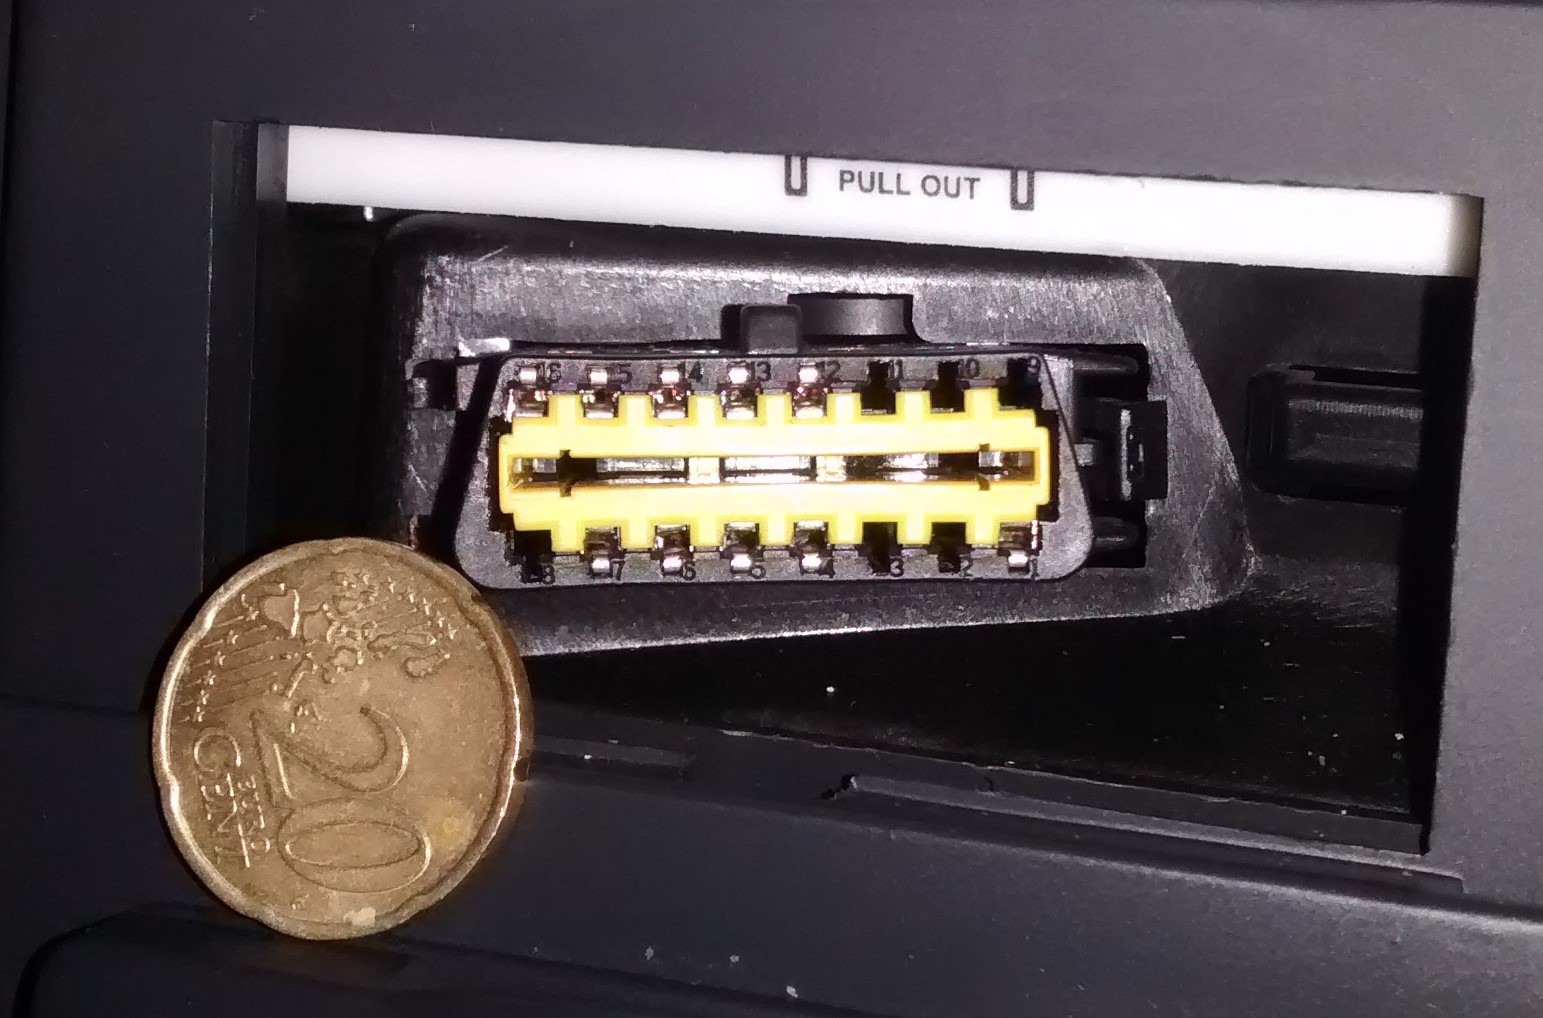
\includegraphics[width=\textwidth]{OBD.jpg}
				\caption{OBDII Port - 20 cent coin for scale}						
				\label{fig:OBDport}
			\end{minipage}
			\hfill			
			\begin{minipage}{0.45\textwidth}
				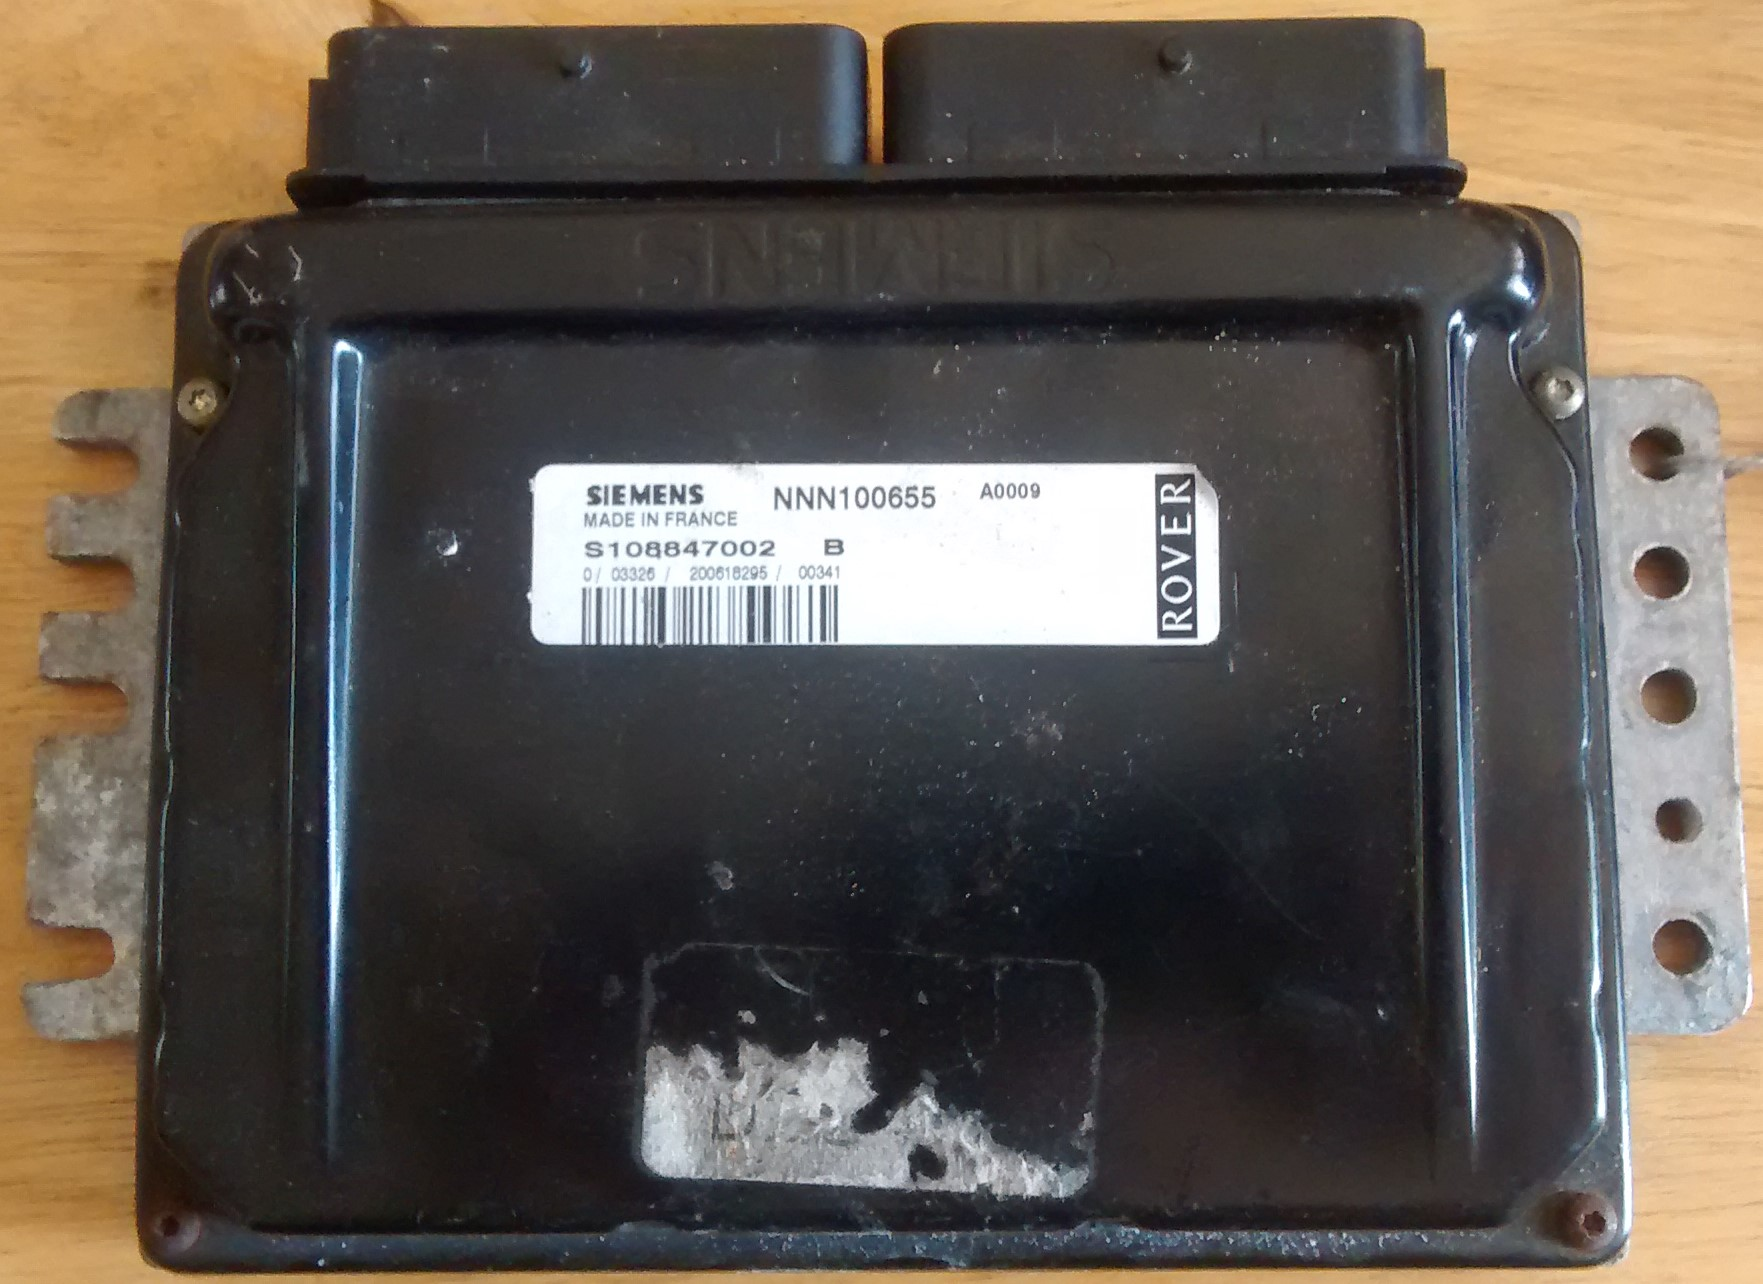
\includegraphics[width=\textwidth]{ECU.jpg}
				\caption{ECU - 20 cent coin for scale}
				\label{fig:ECU}
			\end{minipage}									
		\end{center}
	\end{figure}	
\newpage
\section{OBD Communication}
	\subsection{History}{
		\paragraph{}{
		Due to heavy smog pollution in California, CARB introduced regulations requiring all 1988 and newer vehicles sold in California to be fitted with a system for monitoring the emissions of the vehicle. Unfortunately, this system, later named OBDI, had its shortcomings. While new vehicles allowed for monitoring via diagnostic scan tools, the connection port and its position, as well as the communication protocols, were not standardized, meaning only proprietary scan tools could be used for diagnosis.
		}
		\paragraph{}{
		Prior to the introduction of OBDI, the SAE had proposed a standardised connection port and communication protocols. These changes were taken on board by CARB, and were introduced in OBDII, which was put in force in 1996 in the US. This new system, with it's standardised communication system allowed for generic scan tools to monitor for the vehicle, rather than just proprietary tools.  
		}	
		\paragraph{}{
		Eventually, these regulations reached Europe and European on board diagnostics (EOBD) was introduced. These regulations state that all petrols cars sold in Europe since 2001 and all diesel cars sold in Europe since 2003 must support EOBD. It should be noted that EOBD is the same as OBDII from a technical standpoint.
		}
		\paragraph{}{
		In 2008, regulations were introduced stating that all cars sold in the US must use the ISO 15765 Control Area Network (CAN) communication protocol. A communication protocol defines how data is transferred from the vehicle to the scan tool. This regulation will establish a standard method of communication for all future vehicles.
		}
	}	
	\subsection{Protocols}{
		\paragraph{}{
		The OBDII standards were lenient on how data is transmitted from the vehicle to the scan tool. This lead to vehicle manufacturers creating what they felt was the best way to handle communication. There are now five main communication protocols for OBDII systems.
		\begin{table}[h]
			\begin{center}				
				\begin{tabular}{| l | l |}
				\hline
				\textbf{Protocol} & \textbf{Manufacturer(s)}\\
				\hline
				J1850 Pulse Width Modulation (PWM) & Ford\\
				\hline
				J1850 Variable Pulse Width (VPW) & General Motors\\
				\hline
				ISO 9141-2 & Volkswagen, Audi\\
				\hline
				ISO 14230 Keyword Protocol 2000 (KWP2000) & Chrysler\\
				\hline
				ISO 15765 Control Area Network (CAN) & Toyota\\
				\hline			
				\end{tabular}
				\caption{OBD Protocols}
				\label{tab:Protocols}
			\end{center}
		\end{table}	
		}		
		\paragraph{}{
		Regardless of which protocol a vehicle uses, the process for requesting data is the same. The communication process is handled in hexadecimal format, and starts by selecting a mode. A mode represents a specific function to perform and there are ten in total from 01 to 0A. The functionality of each mode can be seen in Table \ref{tab:Modes} and each will be discussed in sections \ref{ssec:DTC}, \ref{ssec:ClearCodes}, \ref{ssec:Data} and \ref{ssec:OtherModes}. Some modes require a parameter identifier (PID) to be passed, specifying the data item to retrieve. The ECU will send back a response and will have a different conversion method depending on the mode selected. The response will begin with the sum of the mode and $40 _{16}$, for example, if the user requested mode 03, the response would begin with 43.
		}
		\begin{table}[h]
			\begin{center}				
				\begin{tabular}{| l | l |}
				\hline
				\textbf{Mode} & \textbf{Description}\\
				\hline
				01 & Request current powertrain diagnostic data\\
				\hline
				02 & Request powertrain freeze frame data\\
				\hline
				03 & Request emission-related diagnostic trouble codes\\
				\hline
				04 & Clear/Reset emission-related diagnostic information\\
				\hline
				05 & Request oxygen sensor monitoring test results\\
				\hline
				06 & Request on-board sensor monitoring test results\\
				\hline
				07 & Request pending emission-related diagnostic trouble codes\\
				\hline
				08 & Request control of on-board system, test or component\\
				\hline
				09 & Request vehicle information\\
				\hline
				0A & Request permanent emission-related diagnostic trouble codes\\
				\hline
				\end{tabular}
				\caption{OBD Modes}
				\label{tab:Modes}
			\end{center}
		\end{table}		 
		
		\paragraph{}{
		Fortunately, most of the differences between these protocols are low level and do not impact how one can retrieve data from a vehicle using the defined commands. However, there are slight variations when using the CAN protocol.
		}
		\paragraph{}{
		 When requesting DTCs using the CAN protocol, response begins with the number of DTCs, followed by the hex values for each DTC. Using the other protocols, the response only contains the hex values for the DTCs. Mode 05 is unavailable using the CAN protocol so mode 06 must be used as an alternative method to access this data.
		}	
	}
	\subsection{Diagnostic Trouble Codes}{
		\paragraph{}{
		Diagnostic Trouble Codes (DTCs) correspond to faults with a vehicle and are responsible for the illumination of the MIL. Each code begins with an alphabetic letter, indicating the system at fault, followed by four digits specifying the fault. These systems are powertrain, chassis, body and network, represented by the characters P, C, B and U respectively. There are a number of standardized codes, but there are also manufacturer specific codes, which cannot be accessed with generic scan tools.
		}
		\paragraph{}{
		There are three types of DTC: stored, pending and permanent, accessed by mode 03, 07 and 0A respectively. Stored codes represent current issues with the vehicle. These codes can sometimes be fixed by calling the clear codes command on the scan tool. Pending codes represent potential future issues. If there is an irregular data value found by a sensor it may create a pending code. The ECU will continue to monitor this sensor, and if the data value has not returned to the expected value after a certain amount of time, the pending code is converted to a stored code. Otherwise, the pending code will be removed automatically. Permanent codes represent serious issues with the vehicle. These codes are not removed manually by scan tools or automatically by the ECU. In order to remove these codes, the underlying issue that caused the code to appear must be fixed.
		}			
	}
	\label{ssec:DTC}
	\subsection{Clear Codes}{
		\paragraph{}{
		The clear codes function allows one to clear all emissions-related diagnostic information from the ECU and can be accessed by mode 04. This removes stored and pending DTCs, on-board monitoring test results, oxygen sensor data, freeze frame data and data items pertaining to DTC and MIL information, such as distance travelled while MIL is activated. In some cases, clear codes can turn off the MIL permanently. However, if the underlying issues are still present after the clear codes command has been sent, the MIL will illuminate again.
		}
	}
	\label{ssec:ClearCodes}
	
	\subsection{Data}{
		\paragraph{}{
		Emission related data can be accessed via mode 01. This data is retrieved from the sensors and subsystems of the vehicle. In this mode, the user must specify a PID in order to display a certain data item, for example, the PID 0C returns the engine speed.
		}
		\paragraph{}{
		The first step when requesting data is to find the PIDs that are supported for this vehicle, as some vehicles may only support a subset of PIDs. This can be achieved by using PIDs 00, 20, 40, 60 and 80, each of which represent the next 32 PIDs. This will return a hexadecimal value that, when converted to binary, denotes which PIDs are supported. Each bit in the binary string represents a PID. If the bit is 1, the PID is supported and if it is 0 the PID is unsupported.
						
		}
		\paragraph{}{
		As an example, we call 0120, to request the next 32 supported PIDs from 21 to 40. In this example, we receive the hexadecimal response \textit{1A300100}. When this response has been converted to binary, we get the following string:
		\begin{center}
			0001 1010 0011 0000 0000 0001 0000 0000\\
		\end{center}
		The most significant bit represents PID 21 and the least significant bit represents PID 40. If we look at the bits that are set to one, we determine that PIDs 24, 25, 27, 2B, 2C and 38 are supported.
		}
		\paragraph{}{
		Once the list of supported PIDs has been established, the user can request the data for these PIDs. This will return a single data value, so in order for the scan tool to display live data, it must repeat this call. The response must be converted from hexadecimal to the appropriate human readable value, either a string or number. Each PID has a different conversion method, although some PIDs may share them, for example engine coolant temperature and intake air temperature.
		}
	}
	\label{ssec:Data}
		
	\subsection{Other Modes}{
		\paragraph{}{
		Mode 02 allows access to freeze frame data. When a DTC is stored, the ECU takes a snapshot of the values for each available data item. This snapshot is known as freeze frame data. It is accessed and converted in the same way as PID data, although each data item only has one value. It can be used to pinpoint which component is at fault by checking for irregular data values.
		}		
		\paragraph{}{
		Mode 05 allows access to oxygen sensor monitoring test results. These sensors monitor the richness of the air/fuel mixture, which may affect the performance and fuel consumption of the vehicle. Mode 05 is no longer supported in the CAN protocol, but the data can be accessed via Mode 06 instead.
		}
		\paragraph{}{
		Mode 06 allows access to monitoring test results for specific components, such as catalyst monitoring. It can be used as an alternative to Mode 05 to access oxygen sensor monitoring. The user must pass a specific test identifier that is supported by the ECU. The method of finding the supported test identifiers is similar to the process of finding supported PIDs in Mode 02. 
		}
		\paragraph{}{
		Mode 09 allows access to vehicle information. The information available depends on the vehicle, but every vehicle has a vehicle identification number (VIN). This is a 17 character identifier unique to that vehicle, which can be used to search for the history of the vehicle. 
		}
	}
	\label{ssec:OtherModes}

\section{Technology}
	\subsection{ELM327}
		\paragraph{}{
		The ELM327 device, as shown in Figure \ref{fig:ELM327}, used for this project is a compact Bluetooth dongle that can connect to the OBDII port on modern vehicles. The device is relatively inexpensive, with the model used in this project costing {\textsterling}12.95. It supports all OBDII protocols and abstracts the data transfer process by including its own set of commands to handle communication \citep{ELM327}.				
		}
		\paragraph{}{
		The commands that the device supports allow users to either manually or automatically select the protocol, depending on if they know which protocol their vehicle uses. These commands also handle initialization of the device, setting up communication, and formatting the data received from the vehicle. Once the device has been configured, the user can send requests to the vehicle. These requests are in the same format that they are found in the SAE J1979 document, and no further formatting is required.
		}
		\paragraph{}{
		The ELM327 device is easy to set up, without any technical knowledge. The communication set up is handled by the application that it is connected to, so the end user only has to connect the device to the vehicle and the computer that the application runs on. The device is also relatively inexpensive and easy to find on well known retail sites such as Amazon, so it is readily available for users who may not know of specialist retailers for diagnostic scan tools.
		}
		\begin{figure}[h]
				\begin{center}											
					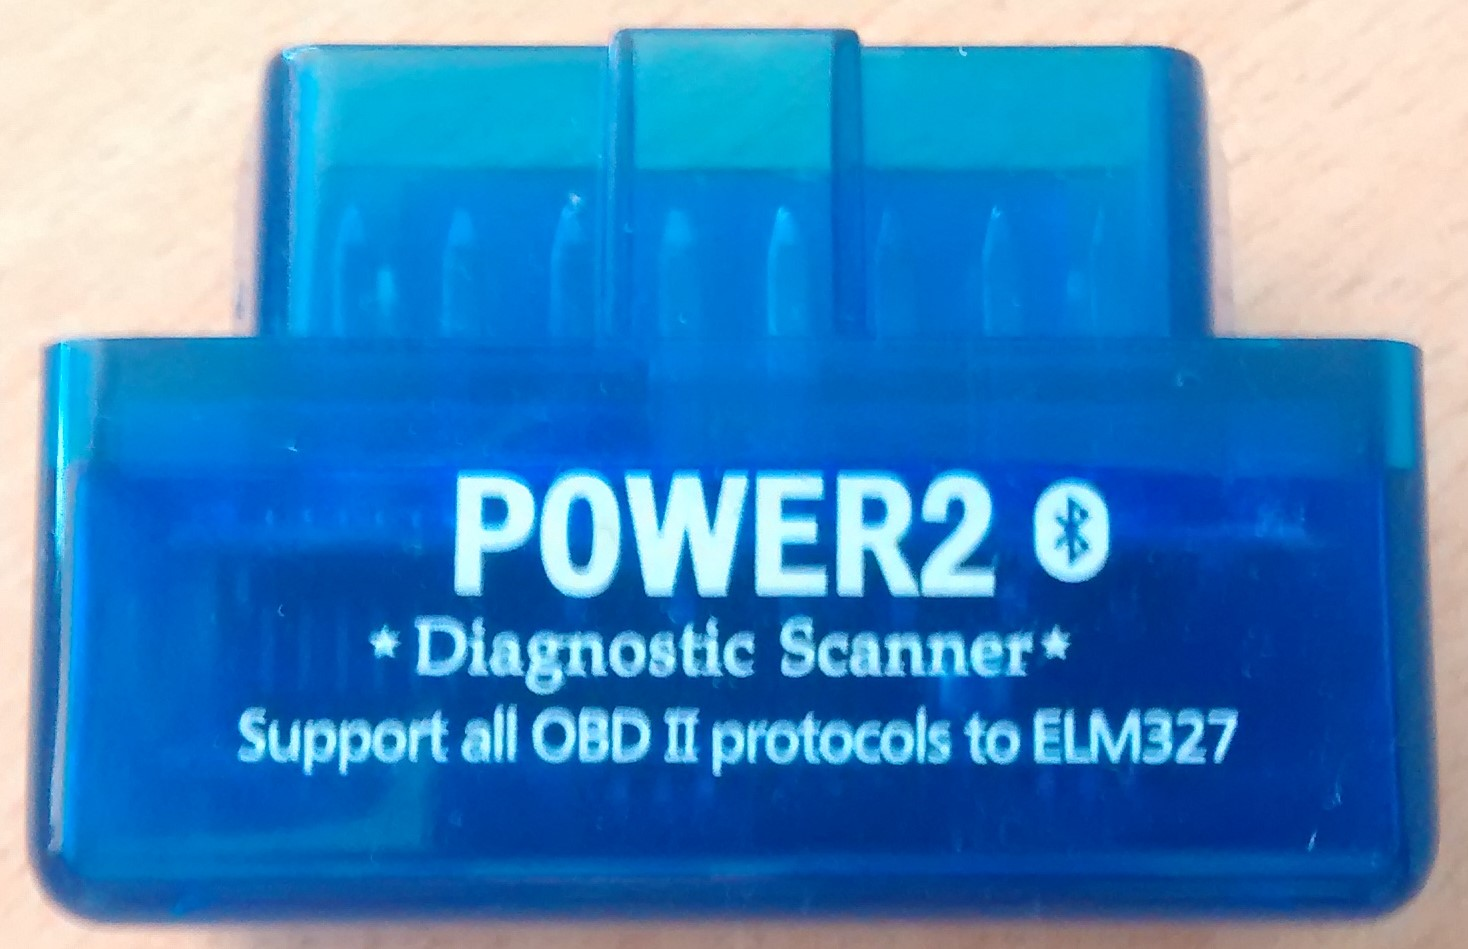
\includegraphics[width=0.4\textwidth]{ELM327.jpg}
					\caption{ELM327 Bluetooth Dongle}
					\label{fig:ELM327}
				\end{center}
		\end{figure}		
\newpage
	\subsection{Windows 10}
		\paragraph{}{
		This project will be deployed on Windows 10 using Microsoft's Universal Windows Platform (UWP). This will allow the application to be deployed on all Windows 10 devices, such as phones, tablets and laptops, using a single code base.
		}
		\paragraph{}{
		Windows is the de facto standard for home users. Most PCs and laptops are sold with Windows pre-installed. Windows 10, the latest iteration of the Windows operating system, is available as a free download to all owners of Windows 7 and Windows 8. Due to it's availability and pricing, it appears that Windows 10 may be a popular choice for home users, and at the time of writing this report there are over 200 million devices running Windows 10 \cite{Win10Nums}.
		}
		\paragraph{}{
		With the release of Windows 10 came the Universal Windows Platform (UWP). This allowed developers to create applications that could be deployed on all Windows 10 devices, without having to create separate code bases. A similar concept was available in Windows 8.1, but it had it's limitations. Deployment was limited to Windows 8.1 phones and Windows 8 tablets/PCs, and there were separate code bases for the phone and desktop/tablet projects, making maintainability and extensibility of the system more complex.
		}
		\paragraph{}{
		The UWP also includes APIs for features such as Bluetooth, printing and WiFi. There is also extensive documentation available for these APIs, allowing the developer to implement systems that work across all devices with relative ease. Microsoft also provides design guidelines for UWP applications, allowing developers, who may not have an in depth knowledge of user interface and user experience design, to create applications with high usability that are aesthetically pleasing.
		}
		\paragraph{}{
		UWP applications can be published through the Windows Store that is accessible on all Windows 10 devices. This allows developers to reach a large user base without concerning themselves with the distribution of the application through multiple markets. Software updates can also be released through the Windows Store, ensuring new features and defect fixes can be deployed to the end user frequently and discreetly.
		}	
		
	\subsection{Xamarin}
		\paragraph{}{
		Xamarin is a framework that can be used for creating native applications for Android, iOS and Mac using the C{\#} programming language. This allows for native Windows applications to be ported to other operating systems, with minimal changes to the code base, creating a portable, extensible and maintainable system.
		}
		\paragraph{}{
		Xamarin allows developers to create applications with the same functionality and UI components of Android, iOS and Mac applications, using a C{\#} codebase. For example, Android UI elements such as buttons will appear and function in the same way as if they were created natively using Java. By creating a shared C{\#} library that contains the core functionality and then creating a platform specific presentation layer for each new operating system, it allows developers to target a large user base with a manageable codebase. 
		}
		\paragraph{}{
		Xamarin can be downloaded through the Visual Studio IDE, allowing Xamarin applications to be developed in the same IDE as the original C{\#} code. This benefits the developer, who does not have to track multiple projects over multiple IDEs. It also means any updates to the Xamarin framework can be downloaded seamlessly, without having to manually check if an update is available and downloading it from an external source. 
		}
		\paragraph{}{
		Xamarin has a developer community on their website, that provides assistance with the development of Xamarin applications. There are a number of guides ranging from the initial setup to performance best practises. Developers can also view Xamarin API documentation and sample applications on how to best use Xamarin and leverage the platform and device specific elements, such as the accelerometer and touch gestures. The website community also has a forum to post questions and find answers from other users, adding more support for the developer.
		}	
%\newpage
\section{Similar Applications}
	\paragraph{}{
	When looking at similar applications, it appeared preferable to look at applications developed using the same technology and deployed on the same platform that the project intended to use. This lead to finding two similar applications available on Windows 10 through the Windows Store. Investigation included finding which modes these applications included, their communication process, the hardware required and the amount of technical information used. These findings are presented in Table \ref{tab:Features}.
	}
	
	
	
	\subsection{Diagnose your car}
		\paragraph{}{
		Diagnose your car is a Windows application available for Windows phones and PCs running Windows 8 and above. It is a paid application, with a free version available that removes some features and includes adverts. When discussing the application in this section, the focus will be on the PC version.
		}
		\paragraph{}{
		The application requires an ELM327 device and a PC capable of Bluetooth connection. The user can find information on the ELM327 in the application, such as where to buy it and how much it costs. The user must pair their ELM327 device with their PC before using the application. Once they have completed this step, they can connect to the device by entering the device name, and the application will automatically connect to it.
		}
		\paragraph{}{
		Diagnose your car allows access to DTCs and diagnostic data in the paid version. In the free version, diagnostic data is omitted and DTCs are displayed without their description. The diagnostic data that is provided is limited to a few generic PIDs, such as engine speed, vehicle speed and engine oil temperature. The data only displays the current value, so it does not track the data values over the period of communication. The application can also display DTCs, run the clear codes command and display the vehicle's VIN and the on/off status of the MIL.		
		}
		\paragraph{}{
		The application attempts to restrict its use of technical terms. For example, the DTCs option is named "Read Defects" and it's icon is that of the MIL, implying that this option correlates to turning off the MIL. However, when the user selects an option, the technical terms begin to appear, with defects now being called stored, pending and permanent DTCs, without an explanation of each type. 
		}		
	\subsection{OBD dash}
		\paragraph{}{
		OBD dash is a free Windows application available for PC. Like Diagnose your car, the application requires an ELM327 device and a PC capable of Bluetooth connection. Information on how to connect the ELM327 device to the vehicle and use it can be found within the application. The Bluetooth device must be paired with the PC before using OBD dash. The user can select their device from a list of suitable paired devices on opening the application.	
		%Modes included, Connection, UI etc
		}
		\paragraph{}{
		OBD dash allows access to DTCs, diagnostic data and vehicle information. PIDs are displayed in dials, similar to those found on the dashboard of a vehicle, and the user can add or remove the PIDs they want to monitor. However, only the current value is displayed, so multiple values cannot be compared over time. DTCs are displayed with their code as well as their description. However, only current and pending DTCs are available through the application. The application also allows the user to view the VIN and protocol that the vehicle supports.
		}
		\paragraph{}{
		Unlike Diagnose your Car, OBD dash uses technical terms frequently throughout the application. It refers to terms such as DTC and VIN without giving an explanation of what they are. While the application does include a help section that directs the user on how to use the application and configure the ELM327 device, it relies on the user having knowledge of protocols and OBD modes.
		%Technical terms
		}
		
		\begin{table}[h]
		\begin{center}				
			\begin{tabular}{| l | c | c |}
			\hline
			\textbf{Function} & \textbf{Diagnose your car}  &\textbf{OBD dash}\\
			\hline
			Mode 01 & Yes & Yes\\
			\hline
			Mode 02 & No & No\\
			\hline
			Mode 03 & Yes & Yes\\
			\hline
			Mode 04 & Yes & Yes\\
			\hline
			Mode 05 & No & No\\
			\hline
			Mode 06 & No & No\\
			\hline
			Mode 07 & Yes & Yes\\
			\hline
			Mode 08 & No & No\\
			\hline
			Mode 09 & No & Yes\\
			\hline
			Mode 0A & No & No\\
			\hline
			Communication process & Bluetooth & Bluetooth\\
			\hline
			Device support & ELM327 & ELM327\\
			\hline			
			\end{tabular}
			\caption{Features of the similar applications}
			\label{tab:Features}
		\end{center}
	\end{table}
\newpage
\section{Architectural Patterns}
	\paragraph{}{
	When considering architectural patterns for the project, it made sense to utilise the model-view-viewmodel (MVVM) architectural pattern. The MVVM architectural pattern is based on Martin Fowler's presentation model design pattern and abstracts the user interface's state from it's behaviour. It was introduced by Microsoft in 2005 to be used with the Windows Presentation Foundation (WPF) platform and is used in UWP development.
			\begin{figure}[h]
				\begin{center}											
					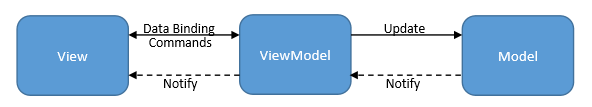
\includegraphics[width=0.75\textwidth]{MVVM.png}
					\caption{Model-view-viewmodel diagram}											\label{fig:MVVM}
				\end{center}
			\end{figure}
	}
	\paragraph{}{
	The model represents the data to be displayed. An example of a model may be a stopwatch. The model can notify the viewmodel of any changes that have been made to the data, such as when the seconds on the stopwatch increase. Likewise, the viewmodel can also update the model with changes made by the view, such as pressing a reset button to set the timer to zero. It is important that the model does not contain logic relating to the user interface, such as formatting strings to appear more aesthetically pleasing.
	}
	\paragraph{}{
	The view represents the user interface and how the end user sees the data found in the model. It manages inputs and events, and notifies the viewmodel of these events. This is accomplished by data binding and commands, which allows properties and functions to be bound to certain UI elements, whilst also separating the logic from the view itself. In UWP, the view is created using Extensible Application Markup Language (XAML).
	}
	\paragraph{}{
	The viewmodel is the liaison between the view and the model. The view may want to update the model, or vice versa, and it must pass these requests to the viewmodel to be handled. For example, a  user may enter text into a field to set a property of the model. This field will be bound to a property on the viewmodel, that will then validate and format the data and pass it back to the model through exposed methods and properties.
	}
	
\section{Conclusion}
	\paragraph{}{
	At the end of the background research stage, information regarding vehicle communication was collected and choices for technology and architectural patterns were able to be made. Overall, the information gathered during this stage served to inform the design and implementation stages of the project.
	% Vehicle Communication, Technology and Architectural patterns
	}
	\newpage

	\chapter{Requirements}
		\section{Introduction}
	\paragraph{}{
	This chapter will outline the functional and non-functional requirements of the project, how they will be supported in the system and the techniques used to capture these requirements.
	}		

\section{Techniques for Requirements Capture}	
	\paragraph{}{
	Traditional techniques \cite{ReqEng}, such as surveys, interviews and analysis of existing documentation and systems, were used to capture the requirements of the system.
	%[SQIRO] - Need to get Object Oriented Systems Analysis and Design using UML
	}
	\paragraph{}{
	The process began with background reading into the domain, as outlined in chapter 2. This involved analysing what functions were available under the OBDII standards, as well as the functions supported by the ELM327 device. Overall, this helped to create a base line for the functional requirements of the project.
	%[Reading - what modes are available, what other tools are there etc.]
	}	
	\paragraph{}{
	Once a list of available functions was compiled, a number of similar applications were analysed. This involved finding which functions were implemented, as well as how they were implemented. The functions that each of these applications supported can be found in table \ref{tab:Features} in chapter 2. By analysing how a function was implemented, it served to highlight which non-functional requirements these similar applications supported and which ones the system should support.
	%[Reviewed similar applications]
	}
	\paragraph{}{
	As the system involved communication with vehicles, it was important to interview people within the motor industry. These people included family members, who have extensive experience in the motor industry, and colleagues that I met during my co-operative education. These interviews were qualitative in nature and the participants were asked what they valued most in a diagnostic scan tool. This served to determine what the system needed from a technical aspect, such as which functions to include in order to effectively diagnose a vehicle. An excerpt of the interview transcript can be seen below:\\
	
	\noindent \textbf{Interviewer: }  Have you used diagnostic scan tools before? \\
	\textbf{Interviewee: }  Yes, I have used them frequently \\
	\noindent \textbf{Interviewer: }  What are the most important diagnostic features of diagnostic scan tools to you? \\
	\textbf{Interviewee: }  DTCs and live data. When I diagnose a car, I will look at DTCs first, then I'll look at live data to check if the DTCs are pointing to a valid issue.\\
	%[Spoke to people in industry - Co-op and family]	
	}
	\paragraph{}{
	Although it was important to interview the domain experts, it was equally important to interview the potential end users. During this stage, proxies for the end user were established. These were vehicle owners with no experience in the motor industry and who had encountered issues with their vehicle in the past. An excerpt of the interview transcript can be seen below:\\

	
	\noindent \textbf{Interviewer: }  What are some of your concerns about using this application? \\
	\textbf{Interviewee 1: }  I would be scared of accidentally damaging my car. I don't have any knowledge about how my car works, so I would be worried about making a mistake and what would happen because of it.\\
	\textbf{Interviewee 2: }  I've never used anything like this before, so I wouldn't know where to start.
	%[Spoke to proxies for the end user / stakeholders]
	}

	\paragraph{}{
	By capturing the expectations of individuals with no technical knowledge, it helped to determine how the functions and results should be presented to the user. As the interviewees voiced their concerns, it became clear that the usability and security of the application were the key non-functional requirements.
	}
	
	\paragraph{}{
	Through the use of reading, observation and interviews, the functional and non-functional requirements of the system were successfully captured.
	%[Conclusion, found a balance between technical needs and user needs]
	}
	
\section{Functional Requirements}	
	\paragraph{}{
	A key outcome of capturing the requirements for this project was determining which OBDII modes to support. Due to the time frame of this project, it was impossible to include all modes, so a subset of modes that would be best suited for the target audience had to be selected.
	}
	\paragraph{}{
	After reviewing similar applications and interviewing domain experts, it was decided that the application would include diagnostic data and DTCs. This corresponds to modes 01, 03, 07 and 0A in the OBDII standard. These modes provide a suitable amount of information to allow a user to diagnose their vehicle, but they also allow the developer to abstract technical information without sacrificing precision.
	}
	\paragraph{}{
	Modes 03, 07 and 0A, representing current, pending and permanent DTCs respectively, provide the means to quickly assess the severity of the issues with the vehicle. The application must display the severity of each DTC type to the end user. If the user needs more information before making a decision, the application must provide additional information on each DTC with minimal use of technical terms.
	}
	\paragraph{}{
	Mode 01, representing current diagnostic data, is more technical than DTCs. However, with the correct level of abstraction and assistance, it can provide the end user with critical information on the issues with their vehicle. The application must display the data in graphical format, so that it can be tracked over a period of time and potentially erroneous or abnormal values must be highlighted for the end user, to assist in their diagnosis.
	}
	\paragraph{}{
	Given the correct guidance, which will be provided by the application, the end user must be able to make an informed decision about the severity of the issues and the cost to repair them, without any technical knowledge.
	}

\section{Non-Functional Requirements}
	\subsection{Portability}
		\paragraph{}{
		To be able to target a large user base, it is important to release the application on multiple systems. For this reason, the system must be portable, so it can be redeployed as an Android or iOS application. To achieve this, the system should leverage the Xamarin framework, and should separate the core functionality of the application from the UI and system dependent features of the application.
		}
	\subsection{Extensibility}
		\paragraph{}{
		Due to the time frame of the project, it is impossible to include all features intended. Also, as new technology becomes available, the application may need to be extended to support it. The system design should consider a modular design where new features, such as supporting a new mode, can be integrated without requiring a restructure of the architecture.
		}
	\subsection{Security}
		\paragraph{}{
		Security can be defined as "a measure of the system's ability to resist unauthorized usage while still providing its services to legitimate users"\cite{SAinP}. As this application is communicating directly with a vehicle, there may be a danger of damage being done to the vehicle and its components. It must be ensured that no harm can be caused by accidental misuse of the application. This will include proper handling of communication, in the event that a user unplugs the ELM327 device during a procedure, as well as providing the user with information on how to use the application correctly.
		}		
	\subsection{Usability}
		\paragraph{}{
		Usability is concerned with how easy it is for the user to accomplish a desired task and the user support the system provides\cite{SAinP}. The application must be intuitive and easy to use for someone with limited technical knowledge of vehicles. This will include limiting the use of technical terms and creating a coherent UI. The application will follow Microsoft's user experience guidelines, so that users of other Windows 10 application will find it easy to use.
		}

	\newpage	

	\chapter{Design}
		\section{Introduction}
	\paragraph{}{
	This chapter will outline the overall system and user interface design of the application. This will include explanations on design decisions made during the project and how the overall design will satisfy the requirements outlined in chapter 3.
	}

\section{System Design}
	\paragraph{}{
	%Intro
	The goal of the system design is to create an extensible and portable application. Any additional core features or aesthetic changes should plug in to the existing system without affecting its current functionality. This can be achieved by applying Martin Fowler's concept of the three principle layers in the design: the presentation layer, representing the user interface, the domain layer, representing the business logic and the data source layer representing communication with another system such as a database.\cite{Fowler}
	}
	\begin{figure}[h]
		\begin{center}
			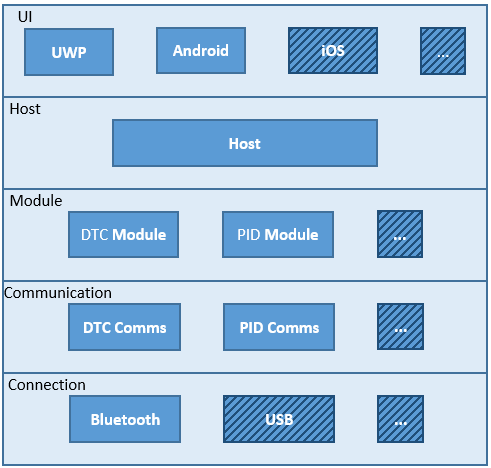
\includegraphics[width=0.5\textwidth]{Architecture.png}
			\caption{System Architecture - Shaded items will not be implemented}
			\label{fig:Architecture}
		\end{center}
	\end{figure}
	\paragraph{}{
	Looking at figure \ref{fig:Architecture}, the UI layer represents the presentation layer, the connection layer represents the data layer and the host, module and communication layers can be combined to represent the domain layer.
	%[EXPLAIN THIS MORE CONCISELY, RE-FACTOR FOLLOWING PARAGRAPHS]		
	}	
	
	\paragraph{}{
	The UI layer represents the user interface and user input handling functionality of the application. Gesture controls, such as swiping, scrolling and pinching are handled and buttons presses are hooked up to the appropriate functionality in the host or module. To port the application to another system, the developer only creates a new UI layer, as the UI is completely abstracted from the core functionality of the system.
	}	
	
	\paragraph{}{
	The host acts as a connection between the core functionality of the application and the UI and user input. The user interface connects to the host, which grants access to the modules that are registered with it. The modules are registered with the host on initialization of the application. This means new modules can be created and added to the application, without requiring a new build.
	\\
	\begin{lstlisting}
// Host Interface
public interface IHost : INotifyPropertyChanged
{
	// List of all Modules associated with the Host
	IList<IModule> Modules { get; }
	
	// The currently selected Module
	IModule CurrentModule { get; set; }
}
	\end{lstlisting}
	}
	\paragraph{}{
	The module represents the model in the MVVM pattern and a core function, such as a mode, in the system. The module contains human readable data that is retrieved from the vehicle. In order to obtain this data, the module must send a request to its communication system. The communication system, which is a part of each module, will take this request and convert it into the corresponding command that the ELM327 device and ECU can understand. It will then send this new request to the connection layer and await a response. This response, in the form of raw hexadecimal data, will be converted into a human readable value by the communication system and returned to the module, ready to be displayed or manipulated.
	\\
	\begin{lstlisting}
// Module Interface
public interface IModule : INotifyPropertyChanged
{
	// The name of the Module
	string Name { get; }
	
	// A list of hints and tips for how to use the Module
	IList<IHelpItem> HelpItems { get; }

	// Initialize the Module
	Task<bool> Initialize();

	// Shut down the Module
	Task<bool> Shutdown(); 
}
	\end{lstlisting}
	}
	\paragraph{}{
	The connection layer represents the low level communication with the OBDII device, such as the ELM327 device. This layer handles the initialization and configuration of the connected device, as well as error handling, such as when the device is disconnected during a procedure or becomes out of range. All requests and responses are handled in hexadecimal format in this layer, allowing the use of raw data to be abstracted from the other layers.
	%Initialization, Setup of device, Handles raw data
	\\
	\begin{lstlisting}
// Connection Interface
public interface IDataConnection : INotifyPropertyChanged
{	
	bool IsInitialized { get; }

	// Logs the command, response and time for each request
	string CommunicationLog { get; }

	// The status of the connected device
    ConnectionStatus DeviceConnectionStatus { get; set; }

	// The protocol of the current vehicle
	Protocol VehicleProtocol { get; }

	// The current connected device
    IDevice CurrentDevice { get; set; }

	// A list of devices the application can connect to
	Task<IList<IDevice>> GetAvailableDevices();

	// Initialize the connection
	Task<bool> Initialize();	

	// Reset the connection
	Task<bool> Reset();

	// Send a request to the device
    Task<string> SendCommand(string command);
}
	\end{lstlisting}
	}

\section{UI Design}
	\paragraph{}{
	It was necessary to create a coherent and highly usable user interface for this application, to satisfy the requirements of the project. This would involve creating a shared look and feel for each module in the application, so that when transitioning from one to the other, the user can easily navigate the user interface and find the functions they need to use with no learning curve.
	%Intro - Created using Pencil
	}	
	\paragraph{}{
	This was achieved by creating a UI shell, as seen in figure \ref{fig:UIShell}, with unified controls and look and feel that would be displayed regardless of which module is currently selected. The shell acts as a means to select and view the current module as well as configure the application, such as which device is connected. Inside the shell, there is a view that the current module will occupy. Each module UI will match the color scheme, font and layout of the UI shell.
	%Microsoft UI Guideline?	
	}
	
	\begin{figure}[h]
		\begin{center}
			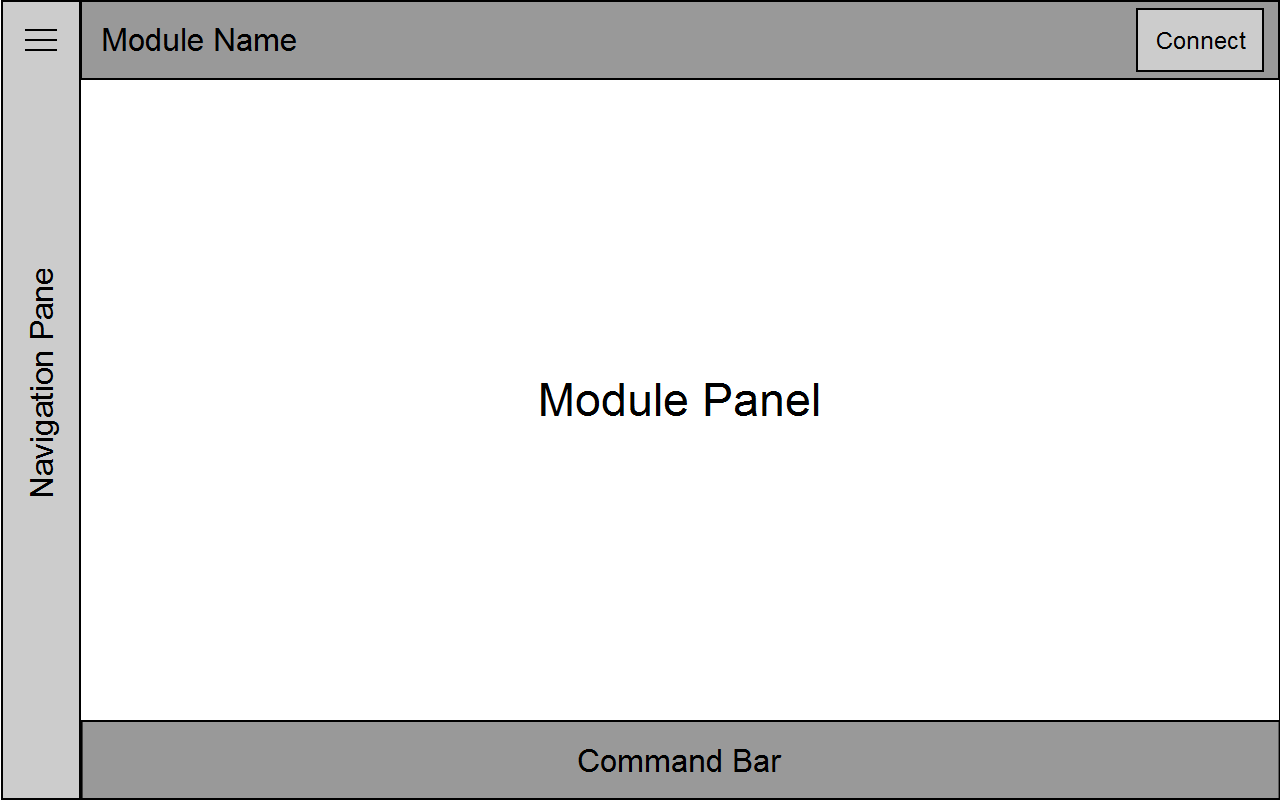
\includegraphics[width=0.5\textwidth]{hostpage.png}
			\caption{UI Shell}
			\label{fig:UIShell}
		\end{center}
	\end{figure}	
	
	\paragraph{}{
	A number of mockups were created for the user interface using an application called Pencil. These were simple wireframes and did not include platform specific UI elements, but instead provide a more abstract view of the overall look and feel of the application. The mockups served as an initial guide when implementing the user interface and as a means of maintaining a coherent and standardised UI. 
	% UI Mockups
	}
	
	\subsection{DTC Module}
		\paragraph{}{						
		% Must display description as well as code, allow the user to clear codes, display additional information, if needed, without interupting flow
		[INTRO]
		}
		\paragraph{}{
		[CODE LIST]
		}
		\paragraph{}{
		[CODE DETAILS]
		% Get more info, without interrupting flow of application. Design chocies include take user to a separate screen, load a modal box, or add a drop down box
		}
		\begin{figure}[h]
			\begin{center}								
				\begin{minipage}{0.49\textwidth}
					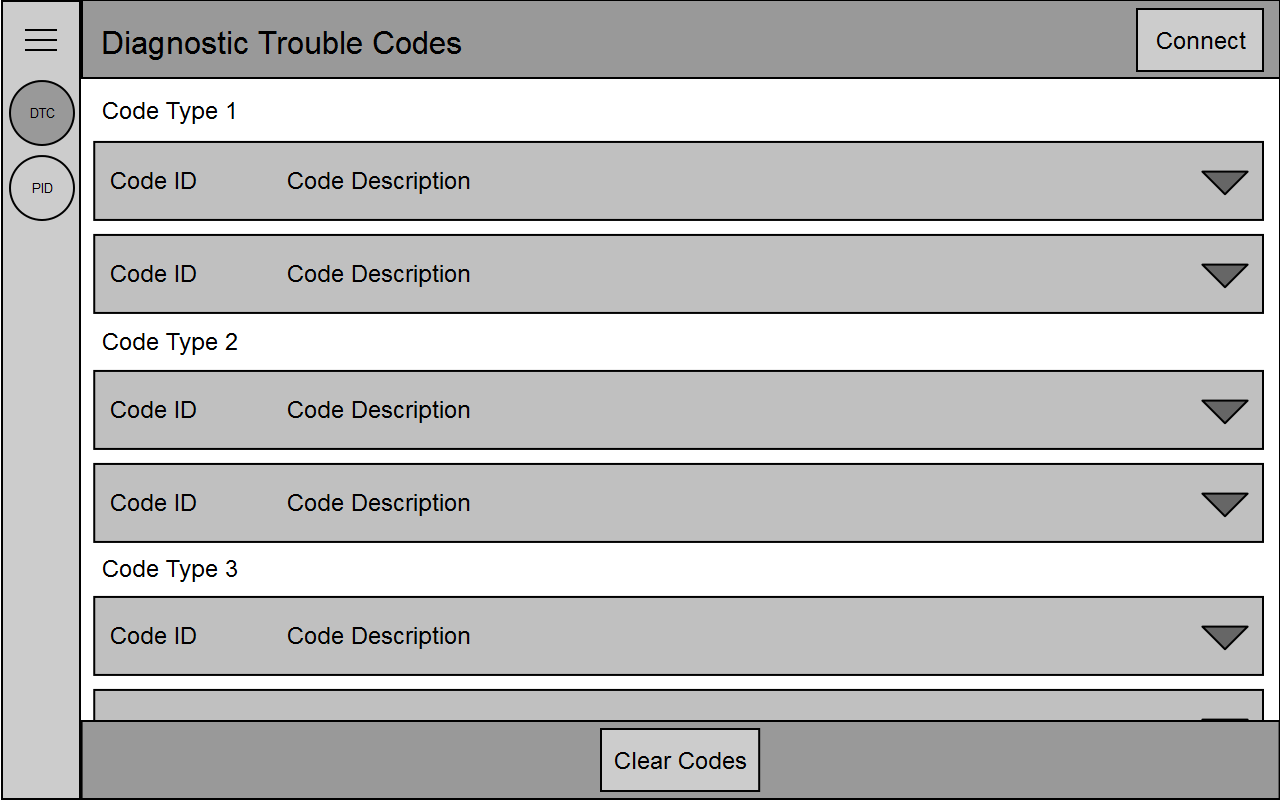
\includegraphics[width=\textwidth]{dtcpage.png}
					\caption{DTC Page}						
					\label{fig:DTCPage1}
				\end{minipage}
				\hfill			
				\begin{minipage}{0.49\textwidth}
					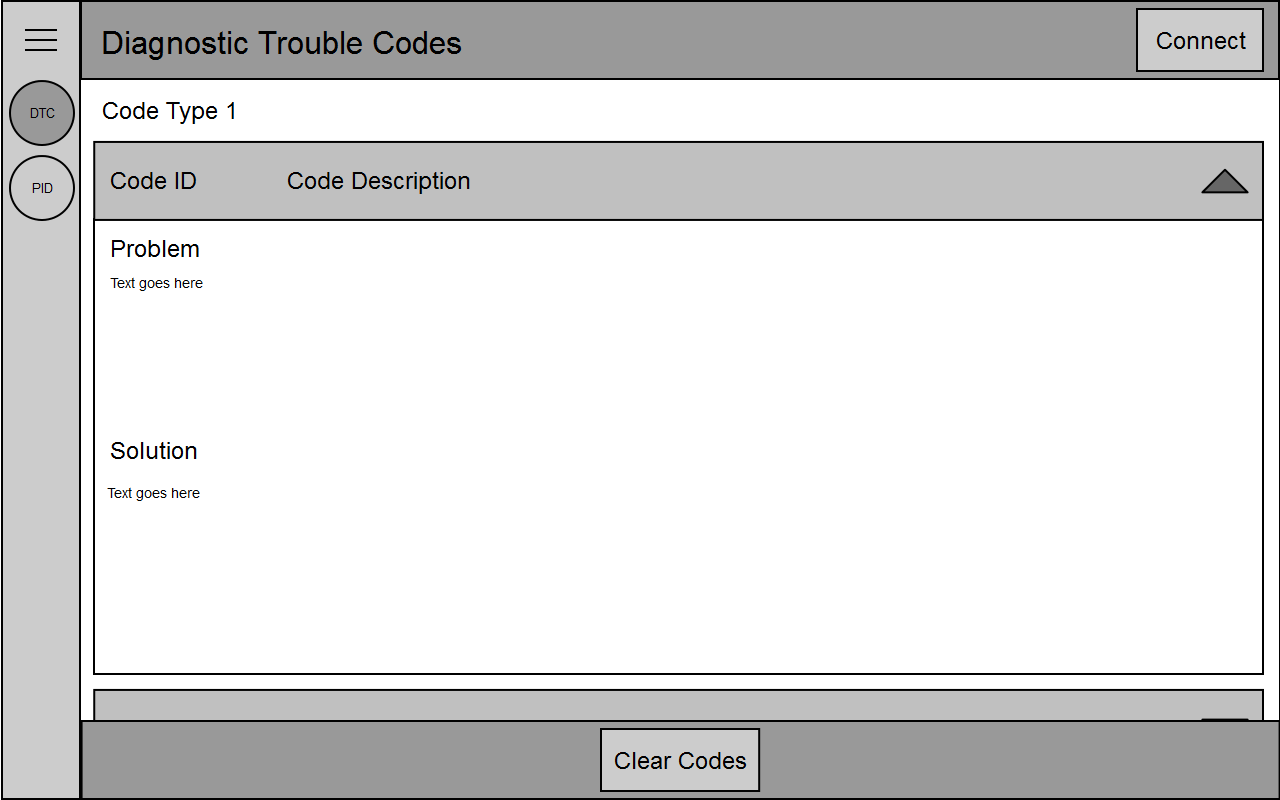
\includegraphics[width=\textwidth]{dtcpage2.png}
					\caption{DTC Page with information}						
					\label{fig:DTCPage2}
				\end{minipage}									
			\end{center}
		\end{figure}
	\newpage
	\subsection{Data Module}
		\paragraph{}{	
		The user interface for the data module consists of two components: data text views and data graph views.  
		% Graphs as well as text, smart graphing, expand and collapse graph, fullscreen graph
		}
		\paragraph{}{
		In the data module, the text views show the current data value in text format, enabling the user to see the current state of the vehicle at a glance. During the design process, displaying the current value on a dial was considered, as seen in the similar applications. This would create a match between the system and real world, as this is how these values are displayed on the dashboard of their car.
		%[TEXT VIEWS] - Considered dials like similar applications
		}
		\paragraph{}{
		However, this approach would lead to the user interface becoming cluttered if a large number of items were on-screen, leading to decreased usability. Instead, a list format was considered, as seen on the left side of figure \ref{fig:DataPage1}. This allowed for a minimalist design that would remain consistent when the number of available pids increased. This approach was eventually selected, as it achieved the same goal of displaying the current value for a pid in a more simplistic and user friendly manner.
		}
		\paragraph{}{
		The key aspect of the data module user interface is the graphing of data values. By graphing the data, the user can track the values throughout the history of current session. 
\\		
		It also provides a more visual representation for the data, allowing the user to identify the maximum, minimum and average values at a glance. As a user may only want to view one particular graph or a subset of graphs, the design allows for user to minimise certain graphs and to set one graph to fullscreen mode for more detailed viewing, as seen in figure \ref{fig:DataPage2}.
		%[GRAPH VIEWS]
		% Smart graphing, the design allow for users to minimise graphs and expand them to full screen
		}
		\paragraph{}{
		The user may want to move forwards and backwards through the data samples that have been collected, to find a particular value. To accommodate this, the design contains controls in the command bar. These include a play and pause button, to start and stop gathering, as well as skip buttons to move through the samples.
		%[CONTROLS]
		}
		\begin{figure}[h]
			\begin{center}								
				\begin{minipage}{0.49\textwidth}
					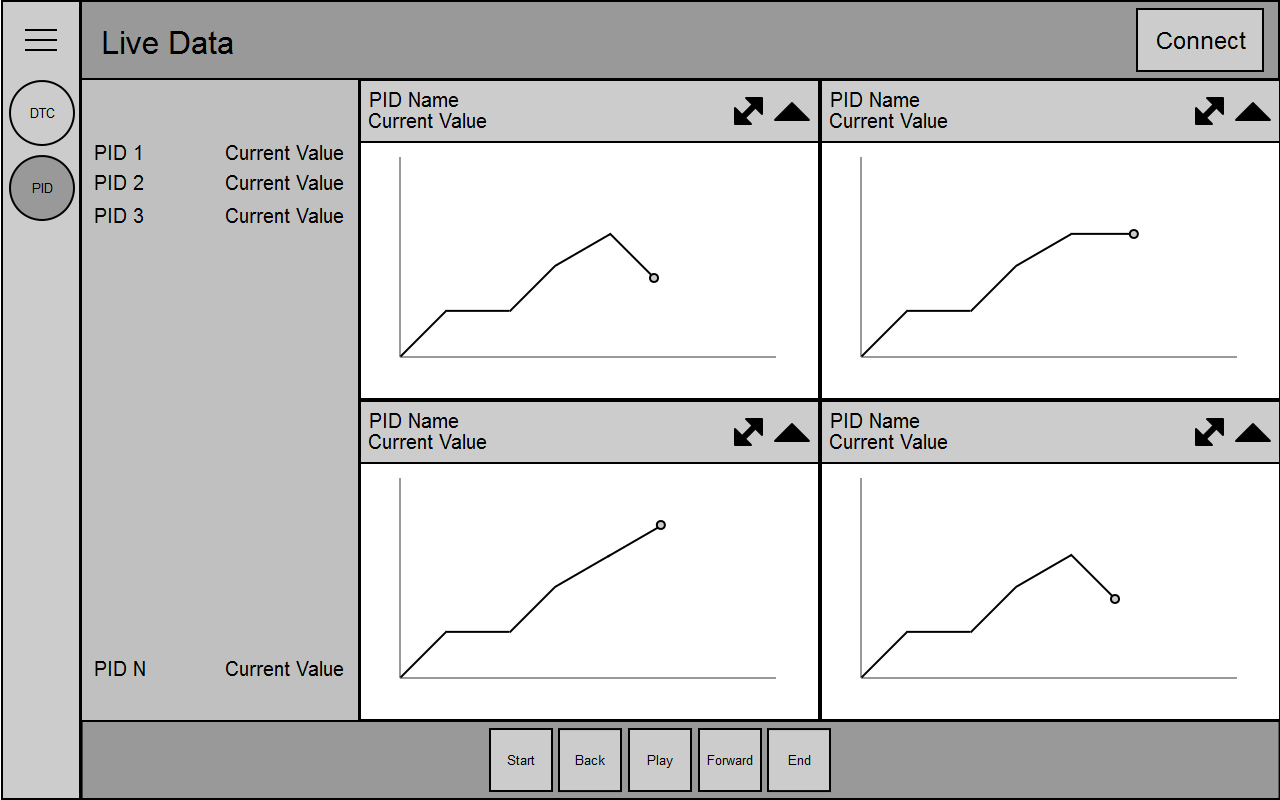
\includegraphics[width=\textwidth]{pidpage.png}
					\caption{Data Page - Graphs Expanded}						
					\label{fig:DataPage1}
				\end{minipage}
				\hfill			
				\begin{minipage}{0.49\textwidth}
					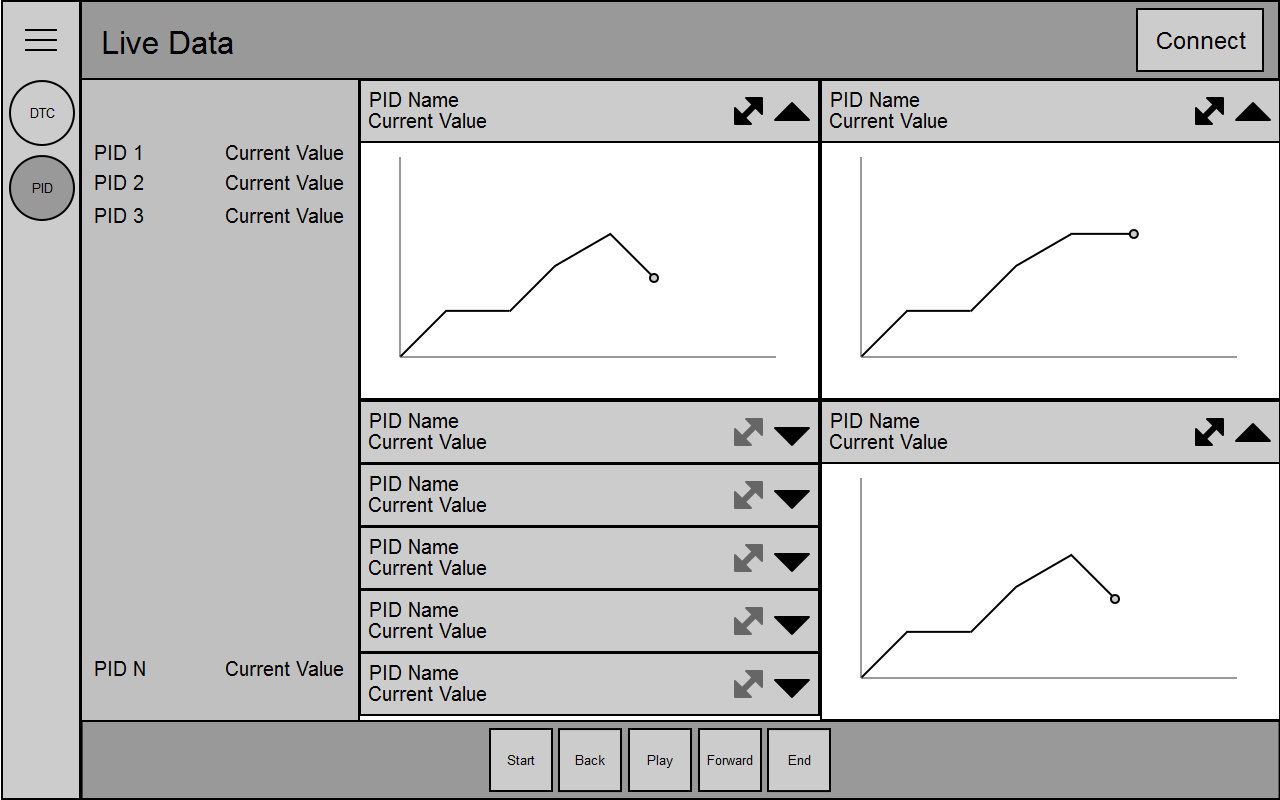
\includegraphics[width=\textwidth]{pidpage2.png}
					\caption{Data Page - Graph Collapsed}						
					\label{fig:DataPage2}
				\end{minipage}									
			\end{center}
		\end{figure}
	
	\newpage
	\subsection{Connection Module}
		\paragraph{}{
		The user interface for connecting to a device was a key component of the project. As this would be the first thing a user would see on loading the application, it had to provide a suitable amount of information, whilst also being minimalist enough as to not confuse the user. There were two design options considered for this user interface. 
		%[Intro]
		}

		\begin{figure}[h]
			\begin{center}								
				\begin{minipage}{0.49\textwidth}
					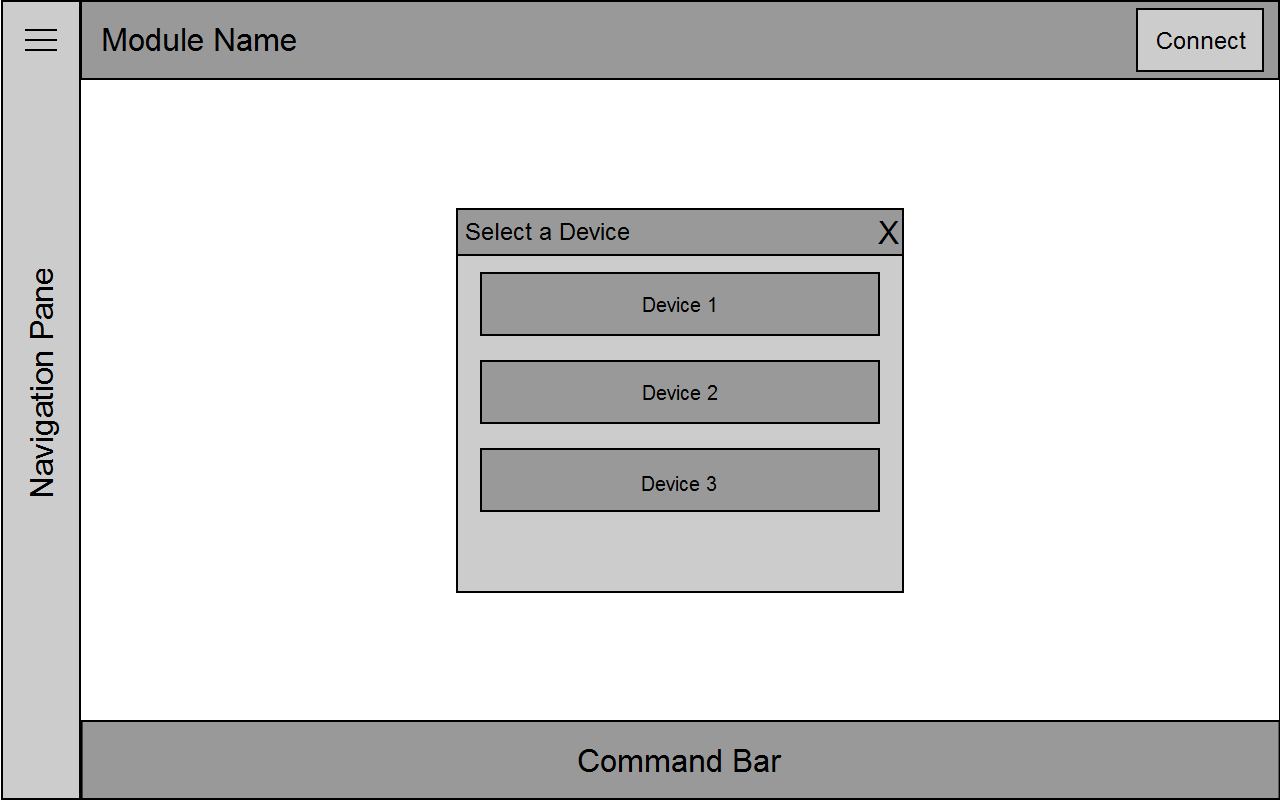
\includegraphics[width=\textwidth]{connectionpage1.png}
					\caption{Connection Design 1}						
					\label{fig:ConnectionPage1}
				\end{minipage}
				\hfill			
				\begin{minipage}{0.49\textwidth}
					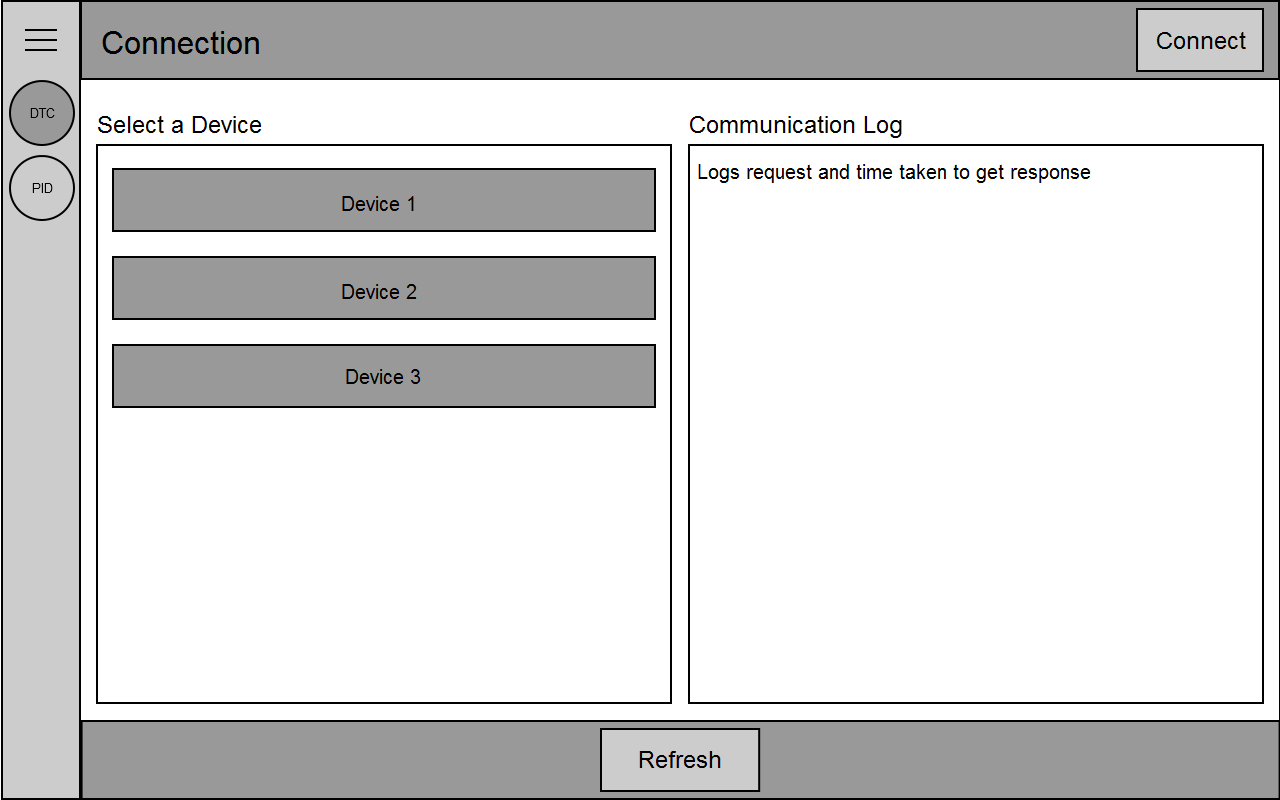
\includegraphics[width=\textwidth]{connectionpage2.png}
					\caption{Connection Design 2}						
					\label{fig:ConnectionPage2}
				\end{minipage}									
			\end{center}
		\end{figure}
		
		\paragraph{}{
		Figure \ref{fig:ConnectionPage1} shows the first design consideration. In this design, a modal box is displayed after clicking the connect button, blocking the user interface behind it. This modal box contains a button for each Bluetooth device paired with the PC. The user can click each button to attempt to connect to the corresponding device. This design is minimalistic and less invasive, as it does not take up a large amount of screen real estate. However, this is also its main drawback, as less space means that only a small amount of instructions can be displayed. As this is the first screen the user will see, they will need to be guided through the setup stages, such as where the ELM327 is connected and how they can pair it to their PC.
		%[Option A]
		}
		
		\paragraph{}{
		Figure \ref{fig:ConnectionPage2} shows the second design consideration. In this design, a module page is created for the connection process. Similar to the first design, the page contains a list of buttons for Bluetooth devices paired to the PC. However, because this design has more screen real estate, a communication log and instructions can be included. The communication log contains information about the communication process, such as any requests that were made and how long it took to receive a response. While this approach allows for more information to be displayed, it requires adding a new module to the existing architecture, so more code is required for this solution.
		%[Option B]
		}
		
		\paragraph{}{
		Ultimately, the second design was used in the final product. While the minimalistic design of the first solution was aesthetically pleasing, it did not match the overall look and feel of the other user interfaces. From a usability perspective, the inclusion of a communication log increased the visibility of the system, allowing a user to see if a request was taking a long time. Overall, the design was selected as it recognised the importance of including instructions on the screen and maintaining a cohesive and visible system.
		%Matched overall deisgn of system, allowed for more information to be displayed to the user on how to connect
		%[Solution]
		}

	\subsection{Home Module}
		\paragraph{}{
		
		}

	\newpage
	
	\chapter{Implementation}
		\section{Introduction}
	\paragraph{}{
	This chapter will outline the implementation and testing process adopted during the project. This will include information on how each component was implemented as well as any issues that occurred during the project and how they were resolved.
	}
\section{Development Environment}{
	\paragraph{}{
	Before starting implementation, a suitable development environment was required. This included a Windows 10 development PC and a method of simulating connection to a vehicle. 
	}
	\paragraph{}{
	A development PC running Windows 10 was required as part of the development environment. It was also preferable that the PC had a touchscreen, to allow testing of gesture controls, such as swipe and pinch, without deploying to a tablet. Fortunately, a Windows 8.1 touchscreen laptop which was eligible for a free Windows 10 upgrade was available before the project began. After the development PC was set up, a suitable Windows 10 tablet to deploy the application on was found. This was a low to middle end tablet, representing what an average user may own.
	}
	\paragraph{}{
	In order to be able to test the application, it needed to connect to and communicate with a vehicle. However, this was not practical as it would require moving from the development environment to the vehicle when testing or debugging the application. Initially, an application that simulated connection to an ECU was bought and used. However, during development it became evident that this would not be suitable for the project. Details about the application and why it was not suitable is discussed in section \ref{ssec:SimSoftware}.
	}
	
	\paragraph{}{
	Instead, an ECU test bench was created (see figure \ref{fig:TestBench}) that could be used as part of the development environment. This consisted of an ECU from a Rover 75 with an OBDII port and a power supply. A specific wiring diagram for the ECU had to be acquired in order to connect the wires to the corresponding pins on the ECU and OBDII port. The ECU test bench can be expanded with additional ECUs to facilitate the testing of communications with multiple communication protocols and vehicle manufacturers.
	}	
	
	\begin{figure}[h]
		\begin{center}										
				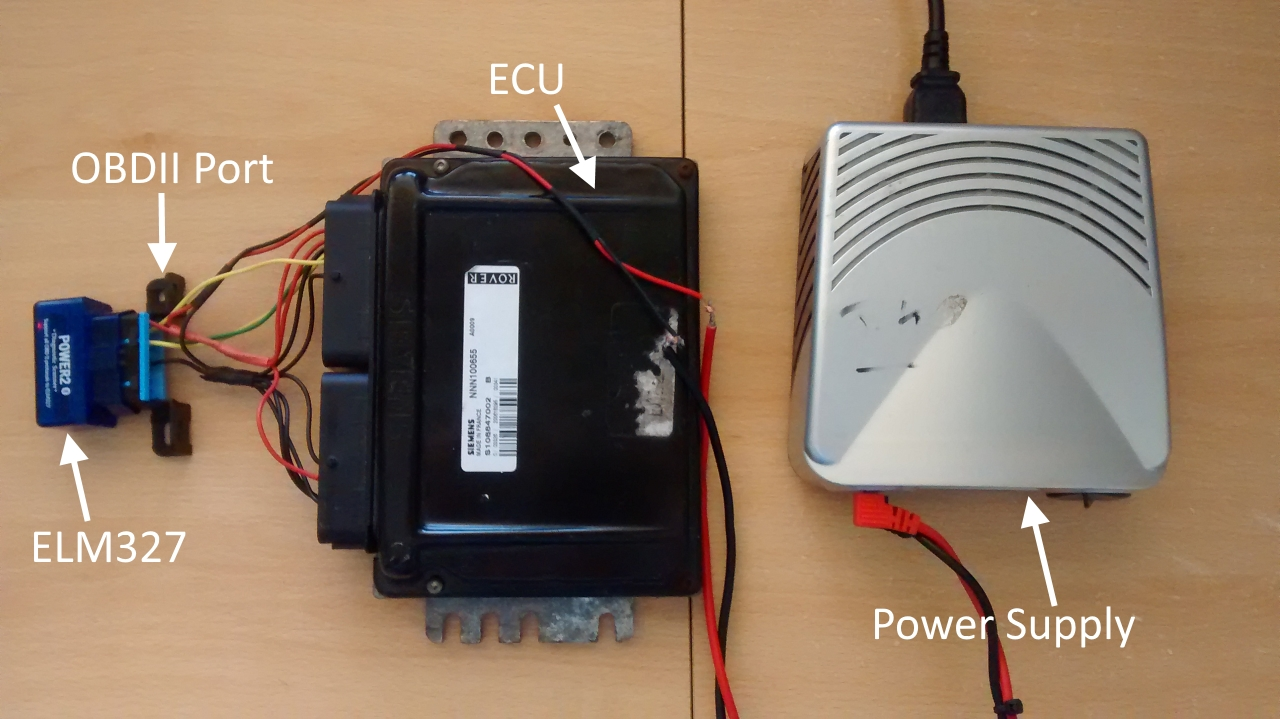
\includegraphics[width=0.8\textwidth]{ECUDesk.jpg}
				\caption{ECU test bench}
				\label{fig:TestBench}
		\end{center}
	\end{figure}
}
\label{sec:DeveEnv}

\section{Prototyping}
	\paragraph{}{
	Prior to starting the project, a lightweight proof of concept was created. This was a C{\#} console application that could connect to an ELM327 simulation application, and display live data on the screen. 
	}
	\paragraph{}{ %Bluetooth API, CAN only
	The application used the 32Feet API by In The Hand Ltd. to handle Bluetooth communication with the ELM327 simulator. The communication system was low level, as it required the address of the laptop and simulator to establish a connection. This was more low level than anticipated and resulted in the hard-coding of the addresses of the development laptop and simulator into the application, which was not optimal. One of the advantages of the 32Feet API, is that the developer can pair Bluetooth devices within their own application. However, this may also be a security issue as an incompatible or harmful device may be paired without the end user's knowledge.
	}
	\paragraph{}{
	The ELM327 simulation software used was an Android application called ECU Engine Pro. The application simulates an ELM327 device connected to an ECU using the CAN protocol. The user can manually add up to six DTCs, and can access the VIN and a limited number of PIDs, such as engine speed. The application displays the address to establish connection via Bluetooth, then the user is taken to the control panel, where they can monitor incoming and outgoing communication logs, as well as edit the DTCs and PID values being returned.
	}
	\paragraph{}{
	The application established communications with the simulator and configured the ELM327 device to use the CAN protocol using the pre-defined commands. The application would then display the first DTC as well as the current engine speed. The values that were displayed were the result of the formatting and converting of the raw data from the simulator.
	}
	\paragraph{}{	
	Overall, the prototype was a success, as it was able to display a DTC as well as the current engine speed on screen. This provided an insight into how communication and data conversion was handled, as well as how to configure the ELM327 device.
	}

\section{Bluetooth Communication}
	\subsection{Description}
		\paragraph{}{
		As the prototype had implemented a subset of the functionality for the communication, it was initially thought that this code code be updated and expanded to create the Bluetooth connection layer. However, during the development process, two key issues became evident, as detailed in section \ref{ssec:BluetoothAPI}. Firstly, the 32Feet Bluetooth API was not supported for UWP applications. Secondly, while UWP applications have their own Bluetooth API, it does not work with the ELM327 simulation software.
		%Implementation of the Bluetooth communication layer of the application began immediately after the setup of the development environment. The goal of this stage was to implement generic Bluetooth communication, such as establishing a connection with the ELM327 device and configuring it, rather than working on module specific communication, such as converting responses. The configuration steps involved resetting the device, allowing the device to auto-detect the communication protocol, turning off echoing of messages and allowing for long responses.
		}
		\paragraph{}{
		Due to these issues, the Bluetooth connection code had to be fully rewritten. This provided some benefits, as the new API is not as low level as the previous one. As seen in figure \ref{code:BTConnectionInit}, connection only requires a device ID, rather than an address of the device and the PC. Another key difference with this API is that the developer can not pair devices through the application. Instead, the user has to pair the device manually before using the application. While this was initially viewed as a limitation, it improved the security of the application, as harmful or incompatible devices cannot be paired with the user's PC. 
		%not as low level as the previous API, More secure
		}
		
		\begin{figure}[h]
			\begin{lstlisting}
// Set up a service for the Bluetooth device
this.service = await RfcommDeviceService.FromIdAsync(this.CurrentDevice.Id);

if (this.service != null)
{
	this.DeviceConnectionStatus = ConnectionStatus.Connecting;
	this.socket = new StreamSocket();

	// Timeout after 5 seconds
	CancellationTokenSource token = new CancellationTokenSource();
	token.CancelAfter(5000);

	try
	{
		// Connect to the socket
		await socket.ConnectAsync(this.service.ConnectionHostName,this.service.ConnectionServiceName, SocketProtectionLevel.BluetoothEncryptionAllowNullAuthentication).AsTask(token.Token);
	
		// Set up the reader and writer using the socket input stream and output stream respectively
		this.writer = new DataWriter(this.socket.OutputStream);
		this.reader = new DataReader(this.socket.InputStream);    		
	}
	catch(TaskCanceledException e)
	{
		this.DeviceConnectionStatus = ConnectionStatus.NotConnected;                            
	}
}
			\end{lstlisting}
			\caption{Establishing a connection to the ELM327}
			\label{code:BTConnectionInit}
		\end{figure}

		\paragraph{}{
		The main component of the Bluetooth connection system was sending and receiving data. As seen in figure \ref{code:BTConnectionSend}, a command is sent to the data writer and appended with a return carriage, to inform the ELM327 that the command has terminated. The reader then attempts to read any incoming messages. However, the length of the  message is unknown and can vary for each command. To deal with this the reader reads one character at a time until a '\textgreater' character appears, signifying the end of the message. If the reader cannot read the entire message, for example, if the user walks out of range of the device, or removes it from the vehicle, the connection will time out.
		% Send & Receive, don't know length of response
		}

		\begin{figure}[h]
			\begin{lstlisting}
// Write
if (this.writer != null)
{
    this.writer.WriteString(command + "\r");
	await this.writer.StoreAsync();
}

// Timeout after 5 seconds                
CancellationTokenSource token = new CancellationTokenSource();
token.CancelAfter(5000);

// Read
try
{
	while (!response.Contains(">"))
	{
		uint size = await this.reader.LoadAsync(1).AsTask(token.Token);                        
        string s = this.reader.ReadString(size);
		response += s;
	}
    
    response = response.Replace(">", "");
}
catch (Exception e)
{
	// Shutdown communication on timeout
	response = NO_CONNECTION;
	this.IsInitialized = false;
}                

if (response.Contains("UNABLE TO CONNECT"))
{
	// Shutdown communication on unable to connect
	response = NO_CONNECTION;
    this.IsInitialized = false;
}

return response;
			\end{lstlisting}
			\caption{Sending a command to the ELM327 and receiving a response}
			\label{code:BTConnectionSend}
		\end{figure}		
		
		%\paragraph{}{
		%There were some issues with the 32Feet Bluetooth API, outlined in section 5.5.1, that lead to the use of Microsoft's own Bluetooth API in it's place. This API allows developers to find all Bluetooth device paired with the PC and choose the appropriate one from the list. Due to the use of this new API, there was less time to work on Bluetooth communication, so the application was created to connect to the first suitable Bluetooth device on the network, with the intention of adding a search function at a later date.
		%}
	\subsection{Issues}
		\subsubsection{Issue 1: Bluetooth API}{
			\paragraph{Description:}
			The 32Feet Bluetooth API used in the prototype was incompatible with the UWP application. This meant that the prototype code that was written for Bluetooth connection could not be reused in the final product.
				
			\paragraph{Occurred during:}
			Week 1
		
			\paragraph{Time taken to resolve:} Half a week to identify the issue, one week to find an alternative solution and one week to implement this solution.
		
			\paragraph{Attempts to resolve:}
			A number of attempts to resolve the issue were made, such as searching for newer versions of the API and researching potential workarounds. Unfortunately, it became evident that the API was completely incompatible with UWP applications, leading to a stand still in development until a replacement could be found.
			
			\paragraph{Solution:}
			Microsoft includes their own Bluetooth API with UWP and this was chosen as a replacement for the 32Feet Bluetooth API. There was an unexpected learning curve that affected the project timeline, but this solution ultimately improved the security of the application and decreased the complexity of the code.
		}
		\label{ssec:BluetoothAPI}
		
		\subsubsection{Issue 2: Simulation software}{
			\paragraph{Description:}
			The replacement Bluetooth API could not connect to the ECU simulation software. This meant connection to an actual vehicle was required to debug and test the application.
			
			\paragraph{Occurred during:}
			Week 1
			\paragraph{Time taken to resolve:}
			One week to find a workaround and half a week to set up ECU.
			\paragraph{Attempts to resolve:}
			Several attempts to contact the developer were made through emails and the Google Play Store, where the application was bought. Unfortunately, no response was received and a decision was reached that the application could not be utilised for this project, as it seemed highly unlikely that the application would be updated to support the Bluetooth API. 
%Looked for other apps
			\paragraph{Solution:}
			To simulate connection to a vehicle, an ECU test bench was created as outlined in section \ref{sec:DeveEnv}. This had an impact on the timeline of the project, as a number of components, such as an ECU and a wiring diagram, had to be sourced as well as assembling the test bench itself. Ultimately, the ECU test bench had the advantage of extensibility over the ECU simulation software, as the latter only supported one protocol, whereas the former can be extended with new ECUs that support various protocols.
		}
		\label{ssec:SimSoftware}		

\section{DTC Module}
		\paragraph{}{
		%Implementation of the DTC module involved creating a UI layer, a module layer and a communication layer for DTCs.	Initially, the DTC module was implemented to only retrieve and display one DTC of each type. This was to quickly test the functionality of the communication system and to provide an impression of the general aesthetics of the module, before implementing it in its entirety.
		}		
		\paragraph{}{
		%The core functionality of this module was to request all current, pending and permanent DTCs and display them on screen grouped by their types. Initially, the module requested current DTCs, and only converted and displayed the first DTC from the response. This code was then reworked to display the first pending DTC and the first permanent DTC. Once the user interface was fully implemented, the module was rewritten to display all DTCs.
		}
		\paragraph{}{
		%Another key aspect of this module was the implementation of the clear codes functionality. The module included a button that, when pressed, issued the clear codes command, then acquired the new list of DTCs and refreshed the UI.
		}
		\paragraph{}{
		%[DTC Info issue]
		}
		
\section{Simulated Communication}
		\paragraph{}{
		While preparing to implement the data module, a potential problem was discovered. While the ECU test bench sent back data that could be graphed, the values were static and could not be changed. This would make it difficult to test the data graphing, as it would require communication with a live vehicle to gather dynamic data values. Instead, a simulation connection class was created.
		%[Preparation for data module, acts like an ECU, behaves like real world (time, responses etc)]
		}
		\paragraph{}{
		The simulation connection class implements the IDataConnection interface seen in figure \ref{code:ConnectionInterface}, but instead of connecting to a Bluetooth device, it handles the requests and returns a response in the format that the ELM327 would use, sending response in hexadecimal format. Because of this, the simulation connection more accurately represents communication with a vehicle and did not require a refactor of the code in the communication layer.
		}	
		\begin{figure}[h]
			\begin{lstlisting}
string response = "NO DATA";

// Request for Data (Mode 01)
if (command.StartsWith("01"))
{
	// Get supported pids
	if (command.StartsWith("0100"))
    {
		// Binary Value: 0001 1000 0111 1000 0000 0000 0000 0000
		response = "410018580000";
	}
    else if (command.StartsWith("0104"))
	{
    	/* Conversion formula: A * 100 / 255 */
    	
    	// Generate a number between the minimum and maximum value
        int min = 0;
		int max = 100;
        Random r = new Random();
		int value = r.Next(min, max);

		// Reverse the equation and convert to hex
        value = (255 * value) / 100;
		response = "4104" + value.ToString("X2");
	}
}
			\end{lstlisting}
			\caption{Simulation connection code for 0100 and 0104 requests}
			\label{code:SimConnectionData}
		\end{figure}

		\paragraph{}{
		As shown in the code fragment seen  in figure \ref{code:SimConnectionData}, a small subset of pids are supported, and each of these pids will return data when a request is made. As each pid has a maximum and minimum possible value, a random value between these two will be generated and this will be the value that the user sees on-screen. The value  is passed through a conversion equation, in reverse order to convert it to hexadecimal format. Finally, the response header is prefixed to this hexadecimal message and is returned to the caller. A more detailed description of how these conversions work can be found in section \ref{ssec:DataModuleDesc}.
		}
		\paragraph{}{
		Due to the success of the simulation connection with respect to the data module, it was expanded to work with the DTC module, returning a set of current, pending and permanent DTCs, as seen in figure \ref{code:SimConnectionDTC}.
		}
		
		\begin{figure}[h]
			\begin{lstlisting}
// Current DTCs
if (command.StartsWith("03"))
{
	// Return P0101, P0121 and P0353	
	response = "43010101210353";
}
// Pending DTCs
else if (command.StartsWith("07"))
{
	// Return P0104, P0132 and P0342	
	response = "47010401320342";
}
// Permanent DTCs
else if (command.StartsWith("0A"))
{
	// Return P0107, P0109 and P0111	
	response = "4A010701090111";
}			
			\end{lstlisting}
			\caption{Simulation connection code for current, pending and permanent DTCs}
			\label{code:SimConnectionDTC}
		\end{figure}

\section{Data Module}
	\subsection{Description}{		
		\paragraph{}{
		[Graphs, List, Play/Pause/Step Controls, Smart Graphing]
		}
		\label{ssec:DataModuleDesc}
	}
	\subsection{Issues}{		
		\paragraph{}{
		[Speed 300ms, down to 170ms]
		[Graph blurring - Smart graphing fixed this but memory was an issue]
		}
		\label{ssec:DataModuleIssues}
	}

\section{Connection Module}
		\paragraph{}{
		[List of paired devices, connection status, comm log]
		}
	
\section{Android Port}
	\subsection{Description}		
		\paragraph{}{
		[Port preparation, MVVM, Bluetooth layer, UI]
		}	
	\subsection{Issues}{
	}
	\label{ssec:AndroidIssues}
\section{Help Information}
		\paragraph{}{
		[Moving help info out of other modules, help shouldn't interrupt modules]
		}
	
\section{Home Module}
		\paragraph{}{
		[Need to implement this]
		}
	
%\section{Performance Re-factoring}
		%\paragraph{}
		%[Module shutdown, limited pids]
		
	
%\section{Issues}
	%\paragraph{}{
	%During implementation, a number of serious issues were encountered that affected the design and development of the project. These issues were resolved, but often required a reconsideration of the initial design decisions.
	%}
	
	%\subsection{Issue 1: Bluetooth API}
		%\paragraph{Description:}
		%The 32Feet Bluetooth API used in the prototype was incompatible with the UWP application. This meant that the prototype code that was written for Bluetooth connection could not be reused in the final product.
		
		%\paragraph{Occurred during:}
		%Week 1
		
		%\paragraph{Time taken to resolve:}
		%Approximately one week
		
		%\paragraph{Attempts to resolve:}
		%A number of attempts to resolve the issue were made, such as searching for newer versions of the API and researching potential workarounds. Unfortunately, it became evident that the API was completely incompatible with UWP applications, leading to a stand still in development until a replacement could be found.
		
		%\paragraph{Solution:}
		%Microsoft includes their own Bluetooth API with UWP and this was chosen as a replacement for the 32Feet Bluetooth API. Aside from the unexpected learning curve, this solution had it's inconveniences, such as not allowing devices to be paired through the application. This meant that there was additional configuration required by the end user. However, this also created a more secure application, as the chance of automatically pairing a potentially malicious device was decreased.
		
	%\subsection{Issue 2: Simulation software}
		%\paragraph{Description:}
		%The replacement Bluetooth API could not connect to the ECU simulation software. This meant connection to an actual vehicle was required to debug and test the application.
		
		%\paragraph{Occurred during:}
		%Week 1
		
		%\paragraph{Time taken to resolve:}
		%Approximately two weeks
		
		%\paragraph{Attempts to resolve:}
		%Several attempts to contact the developer were made through emails and the Google Play Store, where the application was bought. Unfortunately, no response was received and a decision was reached that the application could not be utilised for this project, as it seemed highly unlikely that the application would be updated to support the Bluetooth API. 
		
		%\paragraph{Solution:}
		%To simulate connection to a vehicle, an ECU test bench was created as outlined in section 5.2. This had an impact on the timeline of the project, as a number of components, such as an ECU and a wiring diagram, had to be sourced as well as assembling the test bench itself. Ultimately, the ECU test bench had the advantage of extensibility over the ECU simulation software, as the latter only supported one protocol, whereas the former can be extended with new ECUs that support various protocols.
		
	\newpage

	\chapter{Testing and Evaluation}
		\section{Introduction}
	\paragraph{}{
	This chapter will outline the processes that were utilised to test and evaluate the system developed as part of this project. This will include the testing of functional and non-functional requirements as well as the rating of usability of the application and software quality.
	}
	
\section{Support for Functional Requirements}
	%Two types: Bench testing, real world testing, both capture different things
	\paragraph{}{
	Support for the functional requirements was difficult to evaluate given the domain of the system. This is because the system requires the retrieval of data from a vehicle, which cannot be manually manipulated by the user, for example, by setting a specific DTC or data value. While it is still possible to manipulate some data, for example, pressing the accelerator changes the engine speed value, it would require either a large base of vehicles for testing or the design and creation of a specific hardware device that would act as a configurable ECU, both of which were outside the scope of this project.
	%Intro
	}

	\paragraph{}{
	To counteract this, testing was split into two approaches: bench testing and real world testing. Bench testing utilised the simulation communication system, outlined in section \ref{sec:Simulation}, whereas real world testing utilised live vehicles and the ECU development environment to test the functional requirements of the system. 
	%Bench testing
	}
	
	\paragraph{}{
	Bench testing was utilised for scenarios that required direct and controlled manipulation of data. This was mostly for the testing of user interface elements, such as smart graphing in the data module. Bench testing was carried out on each module in the application to ensure that the information presented to the user on-screen matched what was interpreted from the communication system. Table \ref{tab:BenchTest} shows a subset of the bench tests that were performed.
	
	
	%Bench testing
	% - UI
	% - Extreme scenarios that require control of the values
	% - 
	}
	
	\paragraph{}{
	Real world testing involved connecting to vehicles or ECUs to test the communication system of the application. This approach was utilised to test the functionality of low level communication, such as the Bluetooth connection and data conversion. To verify the outputs of the system, they were compared to those of the similar applications discussed previously in this report. The purpose of real world testing was to ensure the functional requirement of being able to connect to and communicate with a live vehicle was met. Table \ref{tab:RealTest} shows a subset of the real world tests that were performed.
	
	
	% Real world testing
	% - Connection status of ELM327
	% - Converting data from the ECU
	% - Clear codes functionality
	}
	
	\begin{table}[ht]
		\begin{center}				
			\begin{tabularx}{\textwidth}{| X | l |}
				\hline
				\textbf{Test Description} & \textbf{Result}\\
				\hline
				Smart-graphing colours match the data value type & Pass\\
				\hline
				Current value is updated when step forward and step back are pressed & Pass\\
				\hline
				DTC Lists are refreshed after Clear Codes is pressed & Pass\\
				\hline				
			\end{tabularx}
			\caption{Bench Testing Tests}
			\label{tab:BenchTest}
		\end{center}
	\end{table}
	
	\begin{table}[ht]
		\begin{center}				
			\begin{tabularx}{\textwidth}{| X | l |}
				\hline
				\textbf{Test Description} & \textbf{Result}\\
				\hline
				Connection module detects all paired devices & Pass\\
				\hline
				The vehicle communication protocol is correctly identified & Pass\\
				\hline
				All supported pids are returned & Pass\\
				\hline
				Engine speed data value increases when accelerator is pressed & Pass\\
				\hline				
				Pressing Clear Codes removes all Current DTCs from the DTC List & Pass\\
				\hline
				Notification is displayed on application shutdown / sleep & Pass\\
				\hline				
			\end{tabularx}
			\caption{Real World Testing Tests}
			\label{tab:RealTest}
		\end{center}
	\end{table}
	
	\paragraph{}{
	Using these two approaches allowed for the testing of each diagnostic mode that was implemented in the system. This included robust testing of the user interface and the communication systems, which served to verify that the functional requirements of the project had been satisfied. 
	}
	
	%Two approaches to functional testing of the system were taken: bench testing and real world testing. Bench testing utilised the simulation communication system to test functionality that did not directly rely on communication with a live vehicle for validation. This helped to test the UI elements as well as any extreme scenarios in the communication systems. Real world testing utilised live vehicles and the ECU development environment to test functionality relating to connection and communication with a vehicle.	
	%Test each module, test each mode, code was always subjected to regression testing before being committed
	%Regression - If bug was small or caused by changes in the commit, it was fixed immediately, if the bug was larger or due to changes outside of the commit, it was deferred to a later date
	
		
\section{Support for Non-functional Requirements}	
	\paragraph{}{
	The support for the non-functional requirements of the system was evaluated through a number of techniques.
	% Intro
	}
	\paragraph{}{
	The extensibility of the system was measured through the code metrics gathered as part of the evaluation of software quality. A more detailed description of each metric can be found in section \ref{sec:Quality}, however, the overall high maintainability index of the system showcased the extensibility of the architecture.
	% Extensibility
	}
	\paragraph{}{
	The system met the requirement of portability, as the end product was demonstrated to run on both Android and Windows 10 using a shared code base. While it is difficult to quantify the overall portability of the system, it can be determined by the fact that, with the exception of moving the shared code out of the existing UWP project, little to no code changes were required for the core library in order to run the application on Android.
	% Portablity
	}
	\paragraph{}{
	The security of the system was evaluated by ensuring that no damage could be done to the vehicle through accidental or intentional misuse of the application. This was difficult as the system could not be tested on live vehicles due to the implications in the case of the application causing damage to the vehicle. Instead, a number of ECUs were used to mitigate risk. Testing included unplugging the ELM327 device during communication and attempting to connect to the same ELM327 device with multiple tablets. After these tests passed, it was deemed that the requirement of security had been met.
	% Security
	}
	\paragraph{}{
	The usability of the system was evaluated through a usability survey involving domain experts, such as mechanics. The results of the survey were then analysed to determine the overall usability of the system. The process for creating and evaluating the results of the survey is discussed in detail in section \ref{sec:Usability}.
	% Usability
	}
	
\section{Usability Testing}{
	\paragraph{}{
	In order to evaluate the usability of the system, it was important to undertake a usability study with potential users. This study was approved by the Faculty of Science and Engineering Ethics Committee, as shown in Appendix A.
	%[INTRO]
	}
	
	\paragraph{}{
	%[HOW SURVEY WAS CREATED]
	As a significant figure in the area of usability, Nielsen's usability heuristics \cite{Heuristics} were utilised when creating the survey. It was ensured that each usability heuristic outlined by Nielsen could be evaluated by a corresponding question on the survey. The result was a quantitative survey, seen in Appendix B, that asked participants to rate each question from strongly disagree to strongly agree. This allowed for results from each question to be directly compared and to retrieve statistical information about the usability of the application. It was also decided to include a section at the end of the survey, allowing participants to provide feedback on the positive and negative aspects of the application. While this did not fit with the quantitative research approach, this feedback served as a basis for future work on the system.
	%This resulted in the creation of the survey seen in Appendix B. 
	}
	
	\paragraph{}{
	The usability study was conducted on domain experts, such as mechanics, who had previous experience with diagnostic scan tools. Potential candidates were approached and requested to take part in the survey and a time and date for the study was set with the candidates who accepted. On the day of the study, the candidates were given a tablet and an ELM327 device connected to the vehicle. The participants were requested to use the application for up to fifteen minutes and to privately fill out the survey.
	%Potential candidates were approached
	%[HOW SURVEY WAS CARRIED OUT]
	}
	
	\paragraph{}{
	Once all participants had completed the survey, the results were analysed. For the quantitative questions, each answer was transformed into a number between zero and four if the question was positive, such as "I found the look and feel of the application attractive". If the questions was negative, such as "I found the application slow or unresponsive", the answer was transformed into a number between zero and negative four. The average value for each question was calculated to provide an insight into the overall opinion of the usability of the application. The results of this process can be seen in Table \ref{tab:UsabilityScores}.
	
	\begin{table}[ht]
		\begin{center}				
			\begin{tabularx}{\textwidth}{| X | l |}
				\hline
				\textbf{Question} & \textbf{Score}\\
				\hline
				I found the application slow or unresponsive & 0\\
				\hline
				I found it easy to understand the available options on each screen & 3.6\\
				\hline
				I always knew the status of the application & 2.6\\
				\hline
				I felt in control of the application when I was using it & 3.6\\
				\hline
				I found the look and feel was consistent across the application & 3.5\\
				\hline
				I found it easy to recover from any mistakes I made & 3.3\\
				\hline
				I had to go back to the help guide often & -2.3\\
				\hline
				I liked the flow and organisation of the menus / options & 3.3\\
				\hline
				I found it easy to learn how to use the application & 3.6\\
				\hline
				I could understand the information given by the application & 3.6\\
				\hline
				I found the information was displayed in a logical way & 4\\
				\hline
				I found the look and feel of the application attractive & 3.6\\
				\hline
				I found the error messages easy to understand & 3.6\\
				\hline
				I found the instructions and help information useful & 4\\
				\hline
				I found the user input options (buttons, scrolling etc.) did what I expected them to do & 3.6\\
				\hline
			\end{tabularx}
			\caption{Quantitative Results of Usability Study}
			\label{tab:UsabilityScores}
		\end{center}
	\end{table}
	
	%[RESULTS] Information panels on home page were confused for buttons
	}
	
	\paragraph{}{
	The analysis of the results highlighted a few usability issues. For example, during the evaluation it was noticed that the participants frequently mistook the information panels on the home page as buttons that could be used to navigate to the modules and that icons and buttons were too small on the tablet that was used for testing. Despite these issues, given the quantitative analysis of the usability study, it was deemed that the the application was usable.
	%[REFLECTIONS]
	}		
	\label{sec:Usability}
}

\section{Software Quality}{
	\label{sec:Quality}
	\paragraph{}{
	Code metrics were gathered as a means of determining the overall software quality. While the code metrics that were gathered are only a snapshot of the software quality at a single point in time, in this case at the end of the development process, if the code metrics are gathered periodically throughout the development process, they can track the increase or decrease in quality over time.
	}
	\paragraph{}{
	The main tool used to capture the code metrics was Visual Studio. The metrics that are available are lines of code, maintainability index, class coupling, cyclomatic complexity and depth of inheritance. The metrics were run on each project: the Android application, the UWP application and the the core library. The results for each can be found in Tables \ref{tab:AndroidApp}, \ref{tab:UWPApp} and \ref{tab:CoreLib} respectively.
	% Tools used to capture metrics
	% Currently give a snaphot of software quality, but by capturing metrics over time we see quality throughout a project	
	}
	
	\subsection*{Lines of Code}
		\paragraph{}{
		This metric indicates the number of lines of executable code. High numbers may indicate that "a type or method is trying to do too much work and should be split up" \cite{CodeMetrics}.
		}
		\paragraph{}{
		The number of lines of code cannot be used to evaluate the quality of the software alone. However,  by comparing the lines of code between each project, the portability of the system can be evaluated. The significant difference between the lines of code in the core library and the platform specific projects highlight that the majority of the system functionality could be shared between platforms without requiring duplication for each platform.
		%Interpretation
		}
		
	\subsection*{Maintainability Index}
		\paragraph{}{
		Maintainability Index is the measure of the maintainability of the code. It is a numerical value between zero and one hundred, which is then used to determine a rating. Values between zero and nine are given a red rating, indicating low maintainability. Values between ten and nineteen are given a yellow rating, indicating moderate maintainability. Finally, values between twenty and one hundred are given a green rating, indicating high maintainability.
		}
		\paragraph{}{
		As all classes were given a green rating, it can be said that the overall maintainability of the system is high. The classes with the lowest maintainability indexes were the factory classes, such as PidFactory and DataConverter. This is because a lot of the logic is stored within the class. A solution would be to create a database or local file to store this information and retrieve it on request instead of storing it in the class itself.
		%Interpretation
		}
	
	\subsection*{Class Coupling}
		\paragraph{}{
		Class coupling is the measure of "coupling to unique classes through parameters, local variables, return types, method calls, generic or template instantiations, base classes, interface implementations, fields defined on external types, and attribute decoration" \cite{CodeMetrics}. Good software design states that classes should have low coupling. High coupling can indicate "a design that is difficult to reuse and maintain because of its many interdependencies on other types." \cite{CodeMetrics}.
		}
		\paragraph{}{
		The class coupling values were higher in the UWP and Android projects when compared to the core library. This can be attributed to the fact that the UWP and Android projects use the classes that are defined in the core library. In the core library, class coupling is lower as it uses primitive and built-in types such as 'string' and 'int' more frequently than user defined classes.
		%Interpretation
		}
	
	\subsection*{Cyclomatic Complexity}
		\paragraph{}{
		Cyclomatic complexity is the measure of "the structural complexity of the code" \cite{CodeMetrics}. Code that has a complex control, or a higher cyclomatic complexity value, may require more tests to achieve good code coverage, making it less maintainable.
		}
		\paragraph{}{
		Overall, the cyclomatic complexity values in the core library was significantly greater than those of the UWP and Android projects. This can be attributed to the fact that all of the business logic is found in the core library. For this reason, there are more conditions to be tested, for example in the DataConverter class, which checks the pid name and the current value, leading to an insurmountable number of paths. Much like the maintainability index, a solution to this would be to create a database or local file and send a single query, rather than using conditional statements.
		%Interpretation
		}
	
	\subsection*{Depth of Inheritance}{
		\paragraph{}{
		Depth of Inheritance represents "the number of class definitions that extend to the root of the class hierarchy" \cite{CodeMetrics}. A higher value represents a deeper hierarchy meaning the code is more difficult to understand where a method or field is defined.
		}
		\paragraph{}{
		As expected, the depth of inheritance values were much greater in the UWP and Android code when compared to the core code. This is because these projects utilise and extend exist classes within their respective frameworks for user interface elements.
		%Interpretation
		}
		

\section{Conclusion}
	\paragraph{}{
	The evaluation of the system, through testing and gathering code metrics for software quality, highlighted that both the functional and non-functional requirements had been satisfied. Furthermore, the usability of the system was evaluated through live field studies with domain experts and the results found that the system had a high level of usability.
	}		
	\paragraph{}{
	}
		
		\begin{table}[ht]
		\begin{scriptsize}			
			\begin{center}				
				\begin{tabularx}{\textwidth}{| l | X | l | l | l | l | l |}
								
				\hline
				\textbf{Package} & \textbf{Class} & \textbf{Lines} & \textbf{MI} & \textbf{CC} & \textbf{Cyc} & \textbf{DoI}\\
				\hline
				Root & AppRoot & 14 & 84 & 9 & 8 & 1\\
				\hline
				Connection & BluetoothDataConnection & 63 & 77 & 24 & 31 & 1\\
				\hline
				\multirow{2}{*}{UI.Codes} & CodesFragment & 32 & 69 & 25 & 16 & 3\\\cline{2-7}
										  & CodeView & 14 & 67 & 7 & 3 & 4\\\cline{2-7}
				\hline
				\multirow{2}{*}{UI.Connection} & ConnectionFragment & 49 & 65 & 32 & 20 & 3\\\cline{2-7}
										  	   & DeviceView & 18 & 78 & 8 & 6 & 5\\\cline{2-7}
				\hline
				\multirow{2}{*}{UI.Data} & DataFragment & 21 & 76 & 25 & 10 & 3\\\cline{2-7}
     							  	     & DataListView & 28 & 63 & 13 & 4 & 5\\\cline{2-7}
				\hline
				\multirow{4}{*}{UI.Host} & HostActivity & 35 & 69 & 36 & 19 & 9\\\cline{2-7}
										 & HostModuleListToggle & 13 & 78 & 5 & 7 & 3\\\cline{2-7}
										 & ModuleListViewAdapter & 17 & 76 & 17 & 7 & 3\\\cline{2-7}
										 & HelpItemsListViewAdapter & 11 & 81 & 11 & 5 & 3\\\cline{2-7}
				\hline
				\end{tabularx}
				\caption{Android Application Metrics}
				\label{tab:AndroidApp}
			\end{center}
		\end{scriptsize}
		\end{table}		
		
		\begin{table}[ht]
		\begin{scriptsize}			
			\begin{center}				
				\begin{tabularx}{\textwidth}{| l | X | l | l | l | l | l |}
								
				\hline
				\textbf{Package} & \textbf{Class} & \textbf{Lines} & \textbf{MI} & \textbf{CC} & \textbf{Cyc} & \textbf{DoI}\\
				\hline				
				Root & App & 36 & 70 & 40 & 11 & 2\\
				\hline
				Connection & BluetoothDataConnection & 64 & 77 & 25 & 24 & 1\\
				\hline
				\multirow{9}{*}{UI} & HostView & 74 & 57 & 55 & 28 & 7\\\cline{2-7}
									& HomePage & 8 & 64 & 17 & 3 & 7\\\cline{2-7}
									& ModuleHintView & 9 & 63 & 6 & 6 & 6\\\cline{2-7}
									& ConnectionPage & 37 & 61 & 42 & 19 & 7\\\cline{2-7}
									& DTCPage & 16 & 70 & 27 & 7 & 7\\\cline{2-7}
									& DTCView & 8 & 77 & 6 & 2 & 6\\\cline{2-7}
									& DataPage & 13 & 72 & 20 & 4 & 7\\\cline{2-7}
									& DataView & 17 & 75 & 18 & 10 & 6\\\cline{2-7}
									& DataGraph & 61 & 57 & 38 & 21 & 6\\\cline{2-7}
				\hline
				\end{tabularx}
				\caption{UWP Application Metrics}
				\label{tab:UWPApp}
			\end{center}
		\end{scriptsize}
		\end{table}		
		
		\begin{table}[ht]
		\begin{scriptsize}			
			\begin{center}				
				\begin{tabularx}{\textwidth}{| l | X | l | l | l | l | l |}
								
				\hline
				\textbf{Package} & \textbf{Class} & \textbf{Lines} & \textbf{MI} & \textbf{CC} & \textbf{Cyc} & \textbf{DoI}\\
				\hline
				\multirow{5}{*}{Connection} & IDevice & 0 & 100 & 0 & 3 & 0\\\cline{2-7}
											& BluetoothConnectionDevice & 10 & 92 & 1 & 7 & 1\\\cline{2-7}
											& IDataConnection & 0 & 100 & 6 & 12 & 0\\\cline{2-7}					
											& SimulationDataConnection & 39 & 82 & 18 & 22 & 1\\\cline{2-7}
											& ConnectionManager & 6 & 93 & 2 & 5 & 1\\\cline{2-7}
				\hline
				\multirow{4}{*}{Host} & IHost & 0 & 100 & 3 & 3 & 0\\\cline{2-7}
									  & Host & 30 & 76 & 13 & 20 & 1\\\cline{2-7}
									  & IHostViewModel & 0 & 100 & 4 & 5 & 0\\\cline{2-7}
									  & HostViewModel & 43 & 75 & 26 & 26 & 1\\\cline{2-7}
				\hline
				\multirow{7}{*}{Modules.Base} & IModule & 0  & 100 & 4 & 4 & 0\\\cline{2-7}
									  		  & IModuleViewModel & 0  & 100 & 5 & 6 & 0\\\cline{2-7}
									  		  & ICommunicationSystem & 0  & 100 & 0 & 3 & 0\\\cline{2-7}
									  		  & IHelpItem & 0 & 100 & 0 & 2 & 0\\\cline{2-7}
									  		  & HelpItem & 7  & 93 & 1 & 5 & 1\\\cline{2-7}
									  		  & HelpItemFactory & 23 & 76 & 6 & 10 & 1\\\cline{2-7}
									  		  & RelayCommand & 20 & 83 & 7 & 11 & 1\\\cline{2-7}
				\hline
				\multirow{11}{*}{Modules.Codes} & ICode & 0 & 100 & 0 & 6 & 0\\\cline{2-7}
											    & Code & 18 & 91 & 1 & 10 & 1\\\cline{2-7}
											    & CodeFactory & 71 & 32 & 2 & 159 & 1\\\cline{2-7}
											    & ICodeViewModel & 0 & 100 & 1 & 5 & 0\\\cline{2-7}
											    & CodeViewModel & 16 & 91 & 2 & 11 & 1\\\cline{2-7}
											    & IDtcCommsSystem & 0 & 100 & 4 & 4 & 0\\\cline{2-7}
											    & DTCCommunicationSystem & 18  & 82 & 13 & 8 & 1\\\cline{2-7}
											    & IDtcModule & 0 & 100 & 5 & 7 & 0\\\cline{2-7}
											    & DTCModule & 52 & 81 & 23 & 23 & 1\\\cline{2-7}
											    & IDtcModuleViewModel & 0  & 100 & 5 & 4 & 0\\\cline{2-7}
											    & DTCModuleViewModel & 75 & 75 & 29 & 46 & 1\\\cline{2-7}
				\hline
				\multirow{4}{*}{Modules.Connection} & IConnectionModule & 0 & 100 & 5 & 4 & 0\\\cline{2-7}
									  		  		& BluetoothModule & 49 & 81 & 20 & 26 & 1\\\cline{2-7}
									  		  		& IConnectionModuleViewModel & 0 & 100 & 5 & 7 & 0\\\cline{2-7}
									  		  		& BluetoothModuleViewModel & 54 & 82 & 21 & 30 & 1\\\cline{2-7}
				\hline
				\multirow{17}{*}{Modules.Data} & IPid & 0 & 100 & 3 & 5 & 0\\\cline{2-7}
											   & Pid & 28 & 90 & 10 & 18 & 1\\\cline{2-7}
											   & PidFactory & 61 & 35 & 2 & 131 & 1\\\cline{2-7}
											   & IDataItem & 0 & 100 & 1 & 4 & 0\\\cline{2-7}
											   & DataItem & 12 & 92 & 2 & 8 & 1\\\cline{2-7}
											   & DataConverter & 113 & 35 & 5 & 158 & 1\\\cline{2-7}
											   & IDataCommsSystem & 0 & 100 & 4 & 3 & 0\\\cline{2-7}
											   & DataCommunicationSystem & 17 & 81 & 14 & 7 & 1\\\cline{2-7}
											   & IDataModule & 0 & 100 & 5 & 6 & 0\\\cline{2-7}
											   & DataModule & 49 & 81 & 25 & 21 & 1\\\cline{2-7}
											   & IDataModuleViewModel & 0 & 100 & 5 & 2 & 0\\\cline{2-7}
											   & DataModuleViewModel & 92 & 80 & 33 & 62 & 1\\\cline{2-7}
											   & IDataViewModel & 0 & 100 & 4 & 9 & 0\\\cline{2-7}
											   & IDataListViewModel & 0 & 100 & 2 & 1 & 0\\\cline{2-7}
											   & DataListViewModel & 42 & 82 & 12 & 29 & 1\\\cline{2-7}
											   & IDataGraphViewModel & 0 & 100 & 2 & 3 & 0\\\cline{2-7}
											   & DataGraphViewModel & 48 & 82 & 11 & 31 & 1\\\cline{2-7}
				\hline
				\multirow{4}{*}{Modules.Home} & IHomeModule & 0 & 100 & 2 & 0 & 0\\\cline{2-7}
									  		  & HomeModule & 21 & 83 & 14 & 11 & 1\\\cline{2-7}
									  		  & IHomeModuleViewModel & 0 & 100 & 2 & 0 & 0\\\cline{2-7}
									  		  & HomeModuleViewModel & 23 & 83 & 14 & 13 & 1\\\cline{2-7}				
				\hline
				
				\end{tabularx}
				\caption{Core Library Metrics}
				\label{tab:CoreLib}
			\end{center}
		\end{scriptsize}
		\end{table}

	}
}

	
	
	%\paragraph{}{
	%Testing of the application is essential in ensuring that the system satisfies the functional and non-functional requirements.
	%}
	%\paragraph{}{
	%Ensuring the application displays the correct data is paramount, as an erroneous data value could cause confusion for the end user. Functional testing will ensure that data is not incorrectly converted by the communication system or incorrectly displayed by the UI. The output of the application will be compared with the output of the similar applications outlined in section 2.4, to ensure there is no disparity. 
	%}
	%\paragraph{}{
	%Unit tests will be written for each component of the application. These unit tests will be run before a change is ready to be committed to the source control repository. If any unit tests fail, that have not failed prior to the implementation of the recent changes, the code will not be committed until the underlying causes have been fixed. This helps to minimise the number of new defects introduced as part of implementing new features.
	%}
	\newpage
	
	\chapter{Discussion and Conclusions}
			\paragraph{}{
	The objectives of this project were outlined in chapter 1. To determine if the project was a success, it must be evaluated to ensure the objectives were completed. 
		\begin{itemize}
			\item \textbf{Allow users to retrieve diagnostic information from their vehicle}\\
			The system that was developed included the ability to connect to a vehicle, establish communication and retrieve diagnostic information. This information was displayed in a format that a non-technical end user could comprehend.
			
			\item \textbf{Develop a highly extensible and portable system}\\
			The system was highly extensible as it was easy to add new modules during development and required little to no refactoring to implement new features. The system was portable, as it was demonstrated to run on both Android and Windows 10 using the same core code. 

			\item \textbf{Ensure the system cannot cause damage to a vehicle}\\
			The system was developed in a secure manner, so that the end user had no direct line of communication with the vehicle. The application ensured that accidental misuse could not lead to vehicle damage. 
		\end{itemize}
	}
	\paragraph{}{
	The key objectives of the project were achieved, as shown above. The project was also entered in a competition for "Most Commercially Viable FYP". The project came in third place overall, further highlighting the success of this project as a potential commercial venture.
	%Objectives were achieved, Won an award
	}
	
	\paragraph{}{
	The implementation of this project is based on:
	\begin{enumerate}
		\item Extensive study of the literature to identify and utilise knowledge necessary for a successful outcome
		\item Sound engineering principles for requirements analysis, architecture specification, and design, leveraging methods, techniques and tools appropriate to the context
	\end{enumerate}
	
	The subsequent codebase exhibits very good support for the quality attributes of interest - extensibility, security, and portability. The product's usability was evaluated in live field studies and found to be highly usable through quantitative research. All aspects of development were subjected to continuous evaluation in order to support continuous improvement. The overall development results from diligent and consistent application through both academic terms and the the intervening holiday period.
	}

	\paragraph{}{
	There are a number of possibilities for future expansions of the project in the form of adding new functionality and porting the system to new platforms.
	}
			
	\paragraph{}{
	As the project implemented a subset of the modes shown in Table \ref{tab:Modes}, there is scope for extension of the application in this area. This will involve holding exploratory interviews with domain experts, such as mechanics, to determine what new features would complement the existing functionality of the application as well as user interface design for these new modules.
	%[ADD NEW MODES]
	}
	
	\paragraph{}{
	As a key aspect of the project was the development of a portable system, there is scope for this application to be ported to a number of new platforms. As Xamarin supports porting to iOS, Mac and older Windows platforms, a decision will be made as to which platform will be used. However, it is likely that iOS will be the next platform for the system, as it would make sense to target all mobile platforms first.
	%[PORT TO iOS]
	}
	\paragraph{}{
	In conclusion, the system has achieved the goals outlined at the beginning of the project and there is both scope and motivation to expand the system in future, through the implementation of new features and deployment on additional platforms.
	}		
	\newpage	
		
	\begin{thebibliography}{10}
		\bibitem{SAE} SAE J1979:  E/E Diagnostic Test Modes (2014) California: SAE International.		
		\bibitem{Cabala} {\v C}abala, M., Gamec, J. (2012) 'Wireless Real-Time Vehicle Monitoring Based on Android Mobile Device', Acta Electrotechnica et Informatica, 12(4).
		\bibitem {FAQ} CARB, (2015). Frequently Asked Questions (FAQ) About On-Board Diagnostic II (OBD II) Systems. [online] Arb.ca.gov. Available at: http://www.arb.ca.gov/msprog/obdprog/obdfaq.htm [Accessed 30 Nov. 2015].
		\bibitem{ELM327} ELM Electronics Inc. (2014) ELM327 AT Commands [online], available: 	http://elmelectronics.com/ELM327/AT{\_}Commands.pdf [accessed 7 Sep 2015].
		\bibitem{Fowler} Fowler M. (2003) ‘Layering’, Patterns of Enterprise
	Application Architecture, Boston: Addison-Wesley, 17{-–}24.
		\bibitem{MVVM} Likness, J. (2010) Model-View-ViewModel (MVVM) Explained - CodeProject. [online] Codeproject.com. Available at: http://www.codeproject.com/Articles/100175/Model-View-ViewModel-MVVM-Explained [Accessed 30 Nov. 2015].
		\bibitem{Xamarin} Xamarin, (2015) Developer Center - Xamarin [online], available: https://developer.xamarin.com [accessed 30 Nov 2015].
		\bibitem{SAinP} Bass, L., Clements, P., Kazman, R. (2003) Software Architecture In Practice, 2nd ed, Addison-Wesley: Boston.
		\bibitem{ReqEng} Nuseibeh, B. and Easterbrook, S., 2000, May. Requirements engineering: a roadmap. In Proceedings of the Conference on the Future of Software Engineering (pp. 35-46). ACM.
Vancouver
		\bibitem{Android} Developer.android.com. (2016). Android Developers. [online] Available at: http://developer.android.com/ [Accessed 18 Jan. 2016].

	\end{thebibliography}	
	\newpage
\end{document}
